%!TEX program = lualatex
\documentclass[aspectratio=169,11pt]{beamer}

\usetheme{Madrid}
\usecolortheme{whale}
\setbeamertemplate{navigation symbols}{}

\IfFileExists{portuguese.ldf}
  {\usepackage[portuguese]{babel}}
  {\usepackage[provide=*,main=portuguese]{babel}}
\IfFileExists{luaotfload-main.lua}
  {\usepackage{fontspec}\setmainfont{Latin Modern Roman}}
  {\usepackage[T1]{fontenc}\usepackage{lmodern}}
\usepackage{graphicx}
\usepackage{booktabs}
\usepackage{xurl}
\newif\ifcombibliografia
\IfFileExists{biblatex.sty}{%
  \combibliografiatrue
  \usepackage{csquotes}
  \usepackage[style=abnt,backend=biber]{biblatex}
  \addbibresource{referencias.bib}
}{%
  \combibliografiafalse
  \expandafter\def\csname citetext@briso_atafona_2021\endcsname{Briso (2021)}
  \expandafter\def\csname citetext@machado2024_dinamica_linha_costa_paraiba_sul\endcsname{Machado et al. (2024)}
  \expandafter\def\csname citetext@mello2018_erosao_atafona\endcsname{Mello, Machado e Rocha (2018)}
  \expandafter\def\csname citetext@simcosta_dados_2026\endcsname{SiMCosta (2026)}
  \expandafter\def\csname citetext@asbpa2011_erosion_control_structures\endcsname{ASBPA (2011)}
  \expandafter\def\csname citetext@coreloc_imagem\endcsname{Dreamstime}
  \newcommand{\textcite}[1]{\csname citetext@##1\endcsname}
}

\title[Sem. Cartografia X]{Seminário de Cartografia X}
\subtitle[Aspectos de Atafona]{Caracterização fisiográfica e aspectos oceanográficos de Atafona}
\author[Carneiro, Gaiani e Elsas]{Israel Carneiro \and Miguel Gayani \and José Mauro Elsas}
\institute[UERJ]{UERJ -- Faculdade de Oceanografia}
\date{2026}
\titlegraphic{
\includegraphics[width=1.65cm]{uerj.jpg}}

\newcommand{\fonte}[1]{\par\vspace{0.2em}{\tiny Fonte: #1}}

\begin{document}

\begin{frame}
  \titlepage
\end{frame}

\begin{frame}{Sumário}
  \tableofcontents
\end{frame}

\section{Caracterização da área}
\begin{frame}{Localização da área de estudo}
\begin{columns}[T,onlytextwidth]
  \begin{column}{0.45\textwidth}
    \centering
    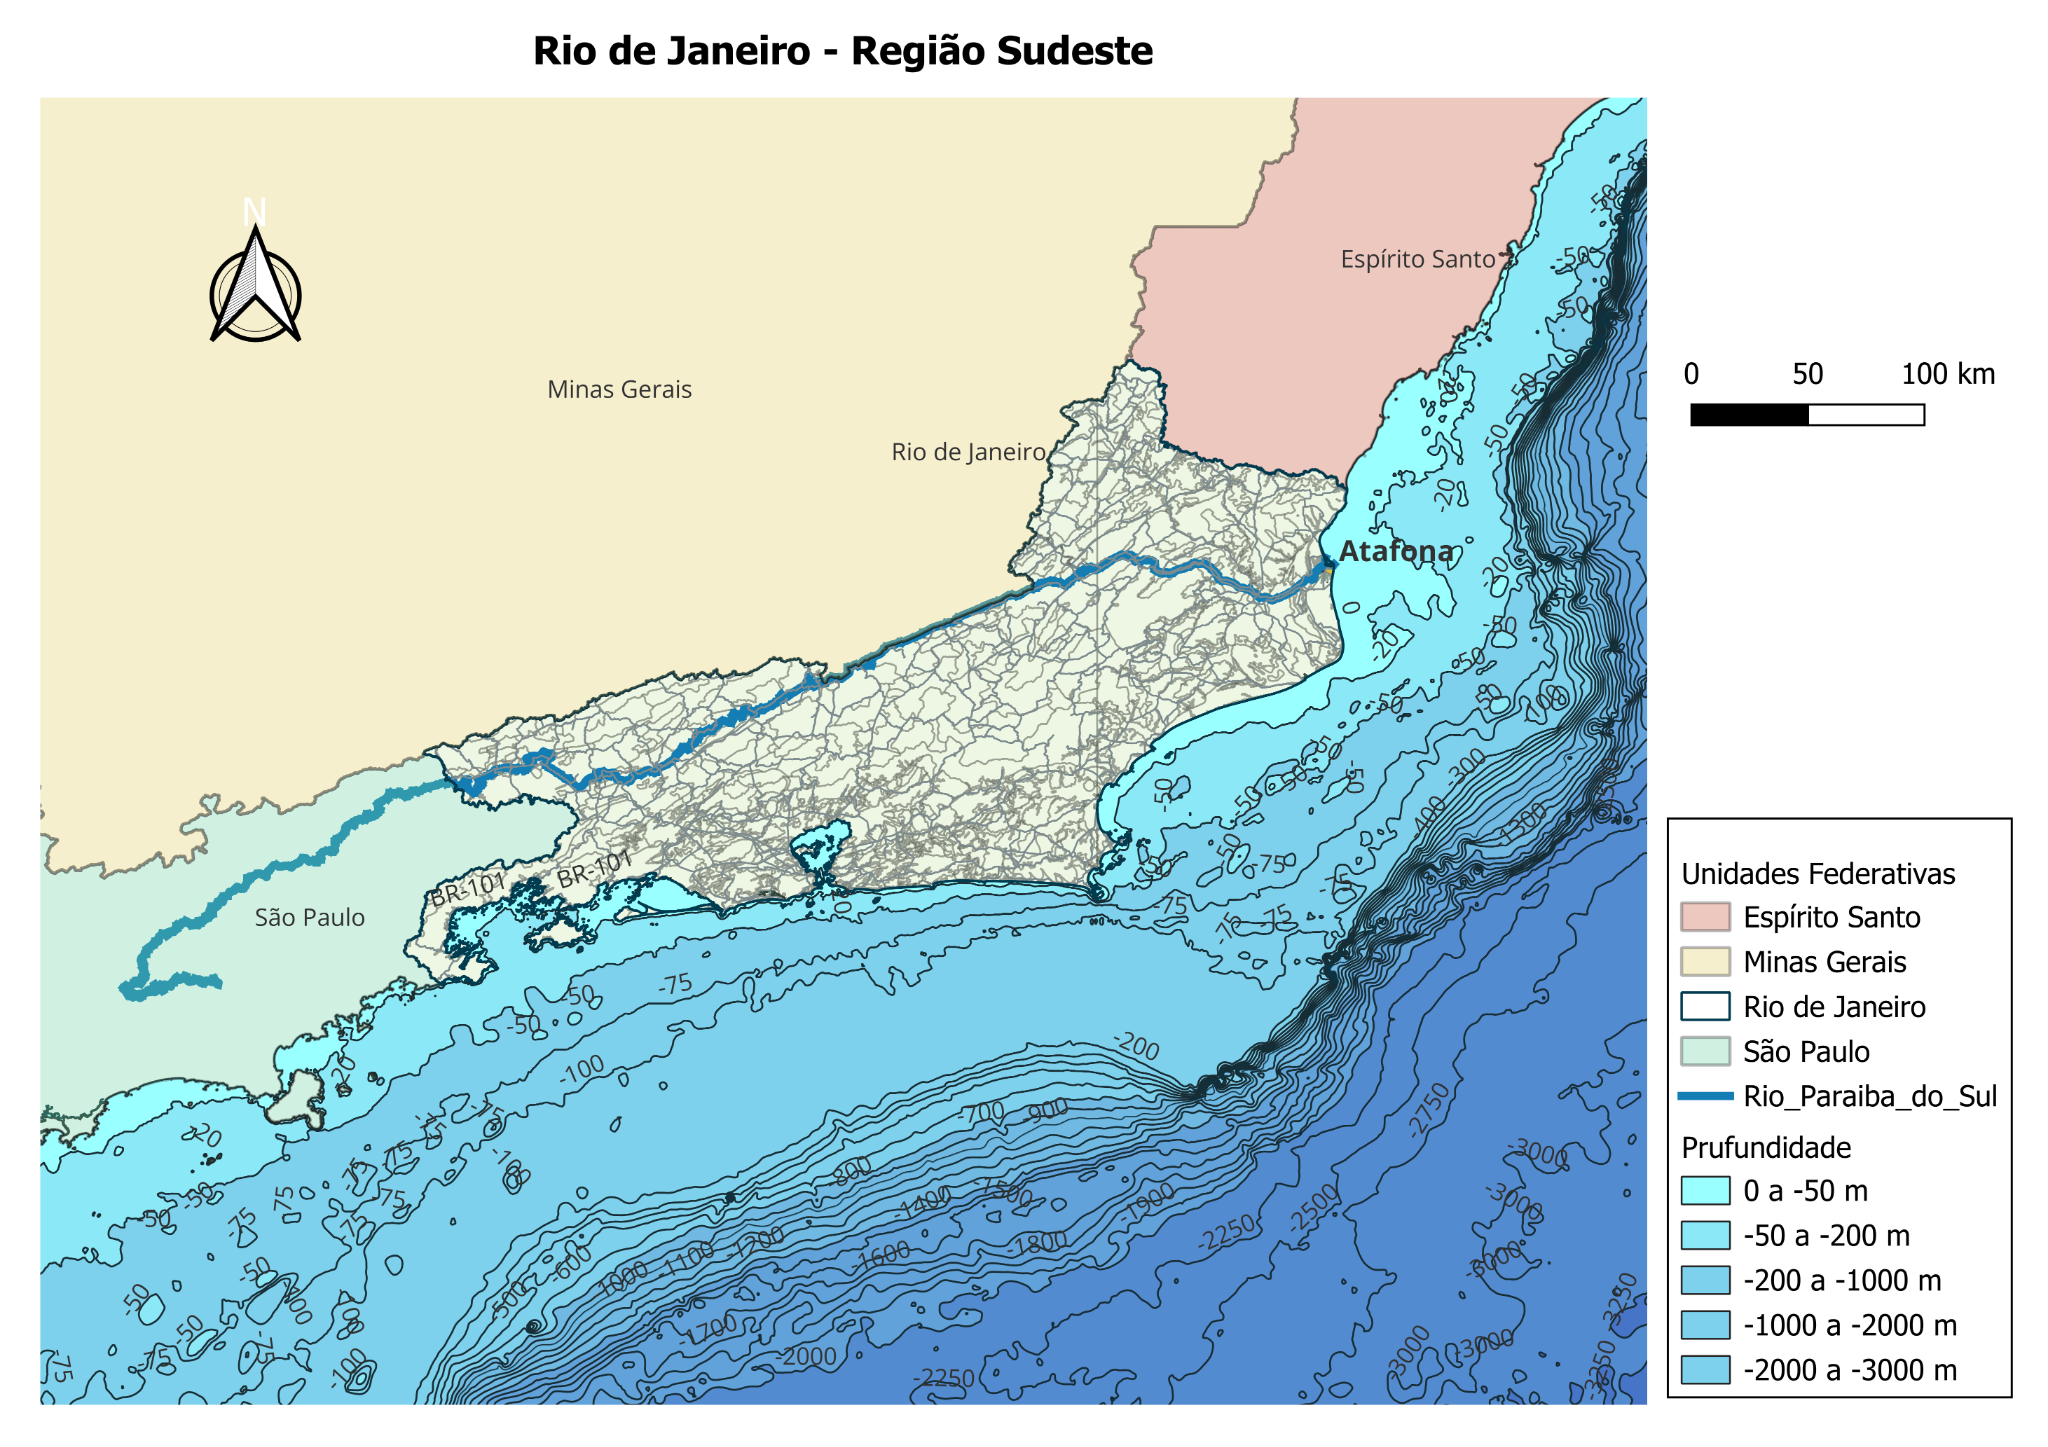
\includegraphics[width=\linewidth,height=0.60\textheight,keepaspectratio]{Estado_Rio_Janeiro.png}
    \fonte{material cartográfico do grupo.}
  \end{column}
  \begin{column}{0.53\textwidth}
    \centering
    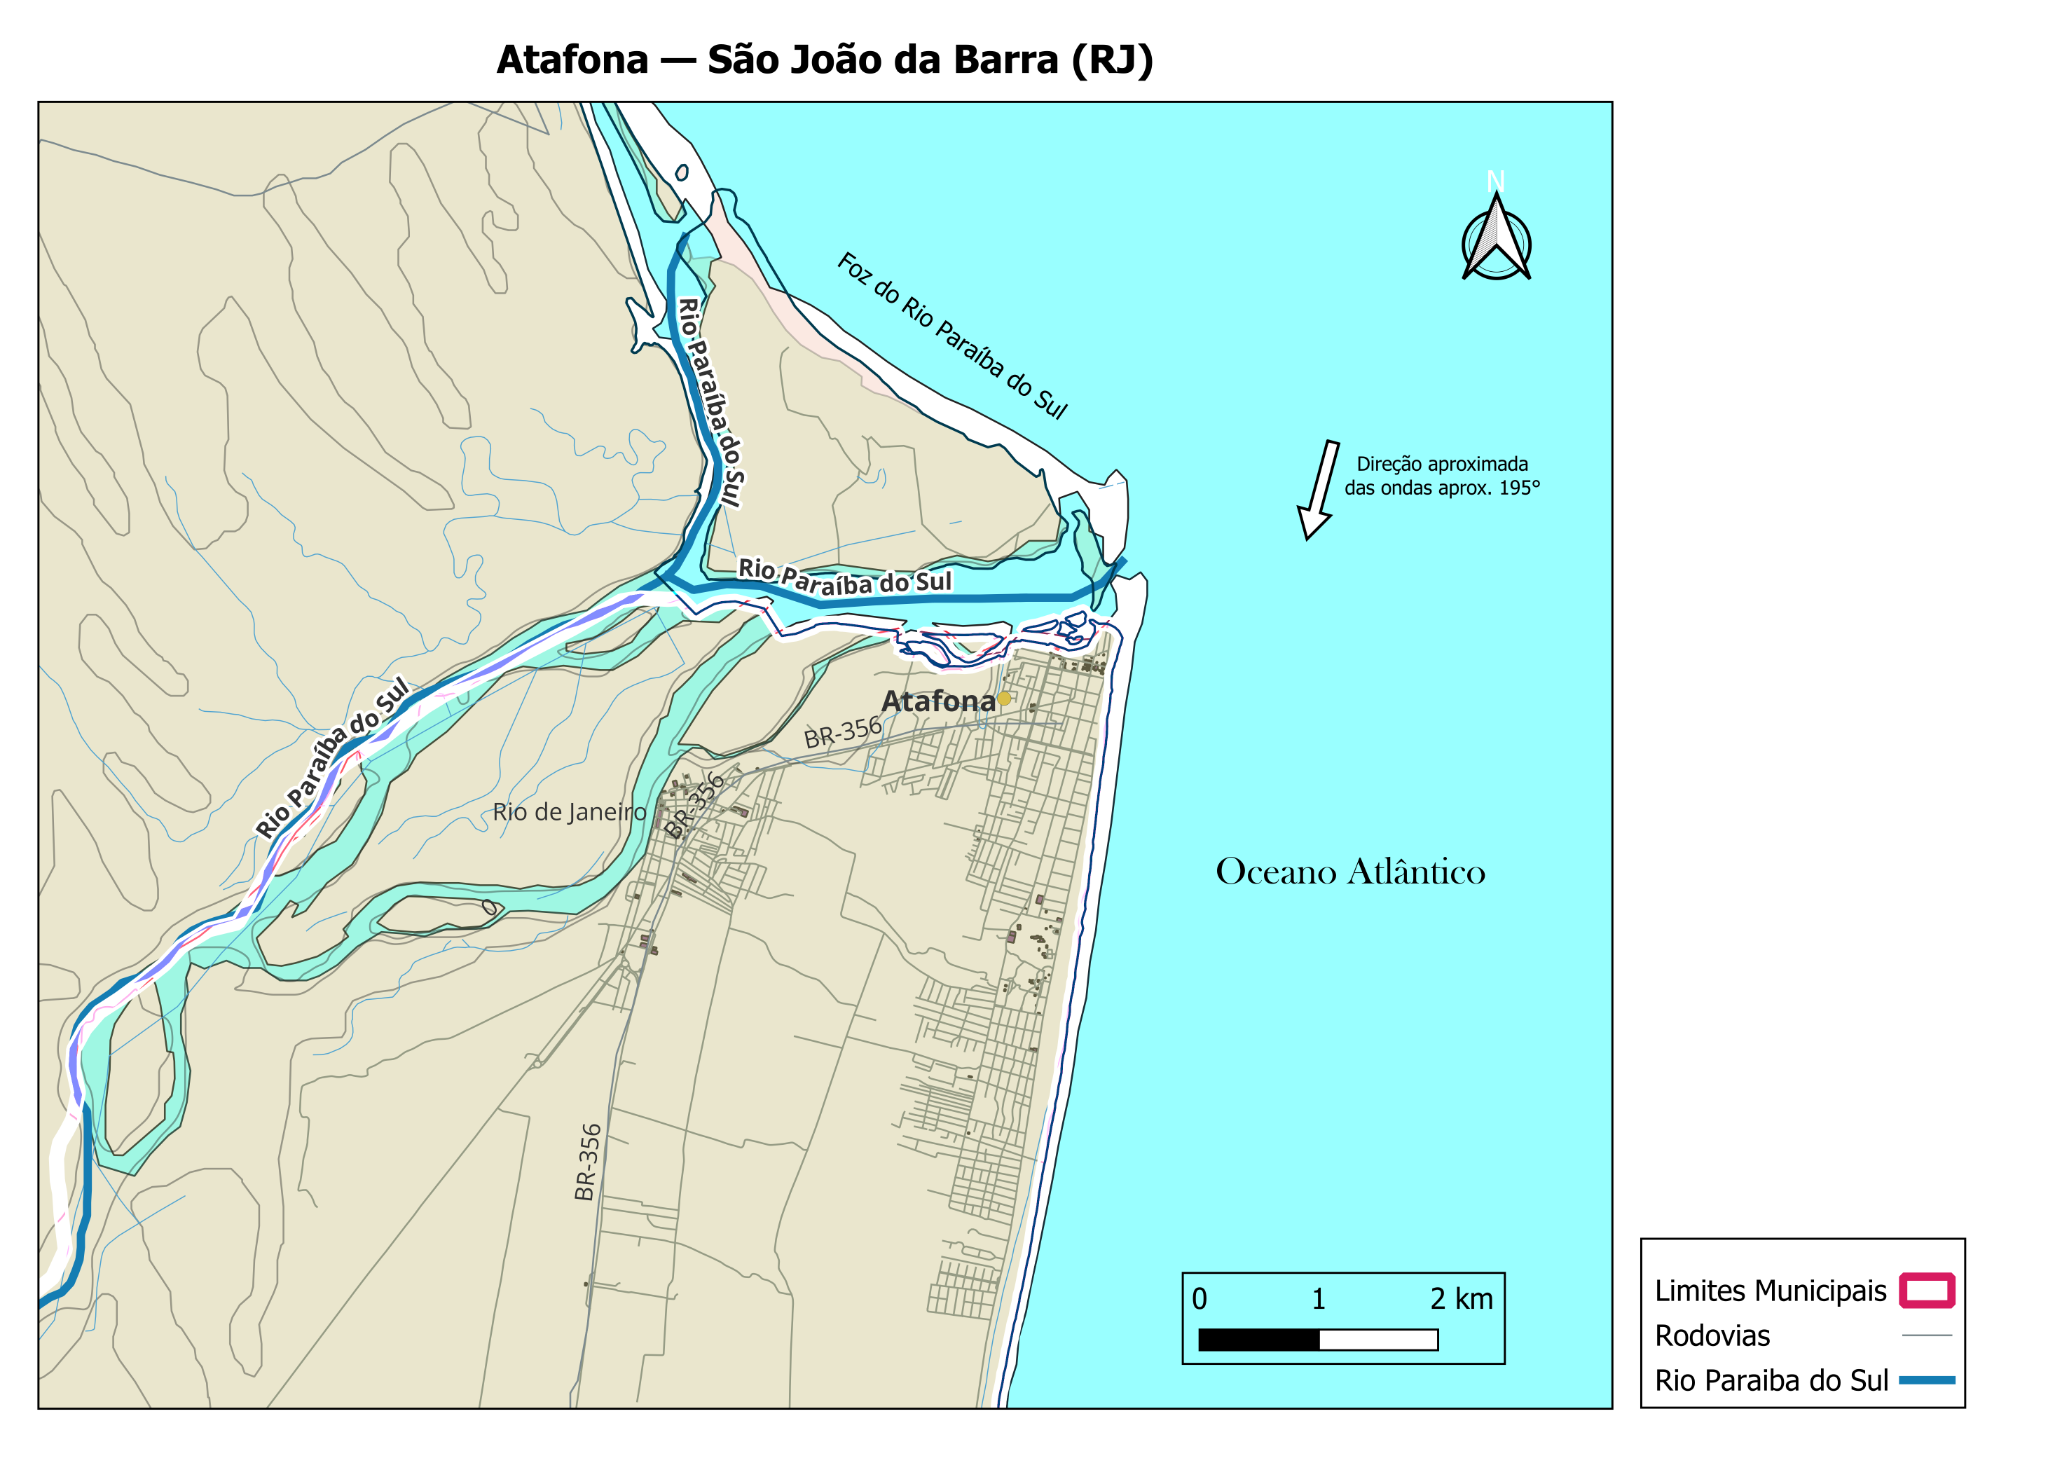
\includegraphics[width=\linewidth,height=0.60\textheight,keepaspectratio]{Atafona.png}
    \fonte{material cartográfico do grupo.}
  \end{column}
\end{columns}
\vspace{0.4em}
\centering
\small Atafona localiza-se em São João da Barra, na margem sul da foz do rio Paraíba do Sul.
\end{frame}

\begin{frame}{Contexto fisiográfico de Atafona}
\begin{columns}[T,onlytextwidth]
  \begin{column}{0.61\textwidth}
    \centering
    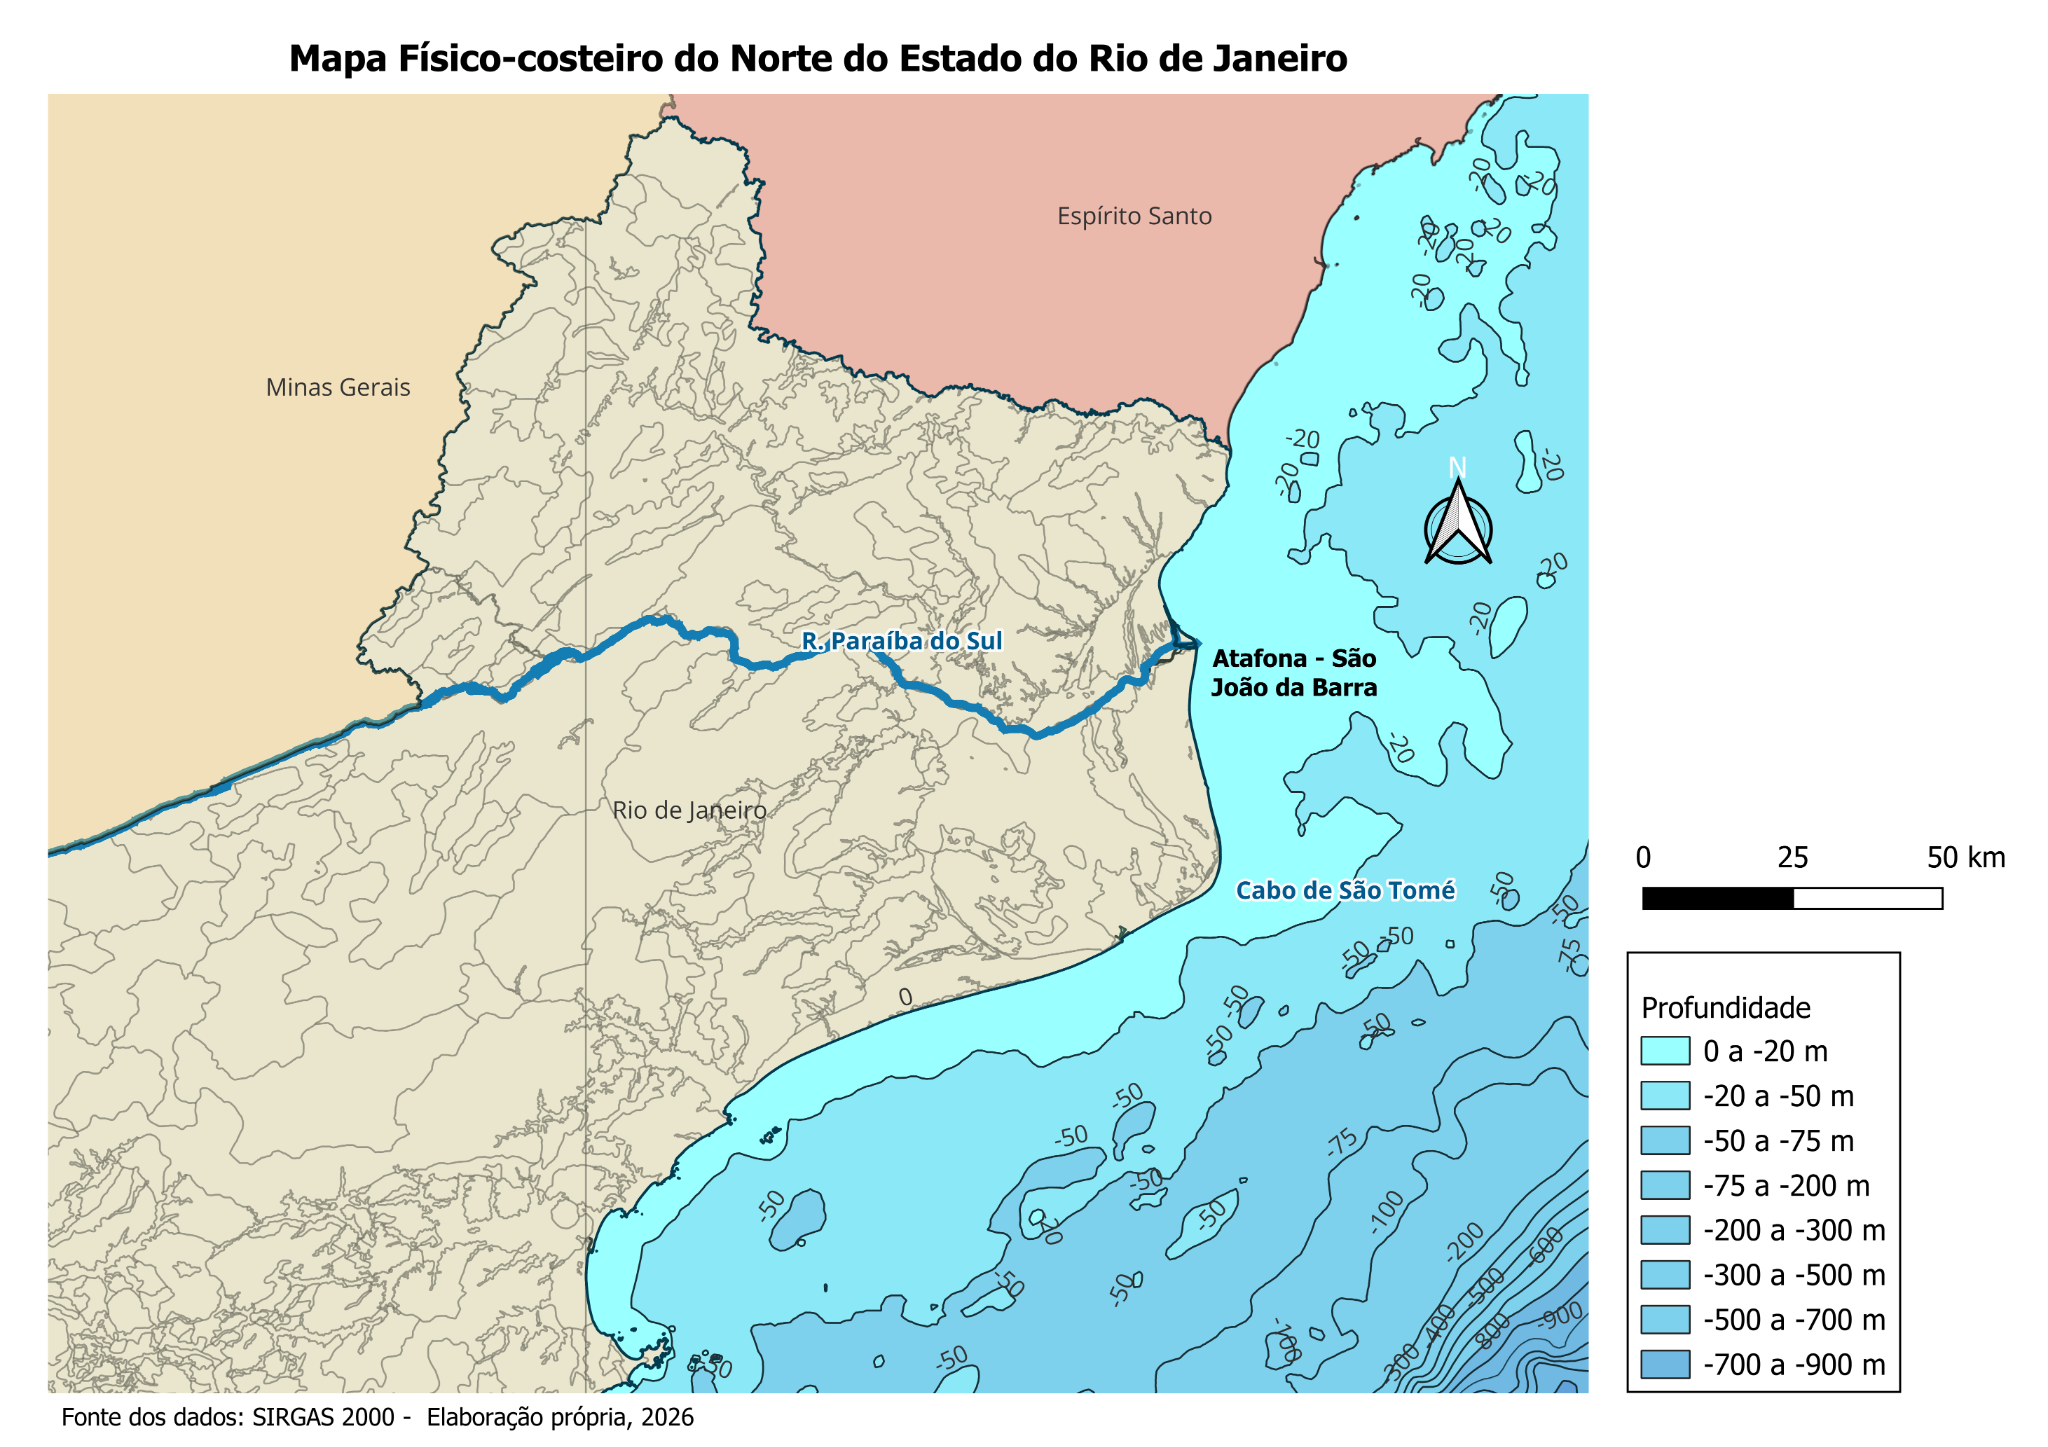
\includegraphics[width=\linewidth,height=0.70\textheight,keepaspectratio]{Mapa_2_Fisico_Costeiro.png}
    %\fonte{material cartográfico do grupo.}
  \end{column}
  \begin{column}{0.35\textwidth}
    \vspace{2.0em}
    \begin{itemize}
      \item planície costeira e deltaica de baixa altitude;
      \item sedimentos predominantemente inconsolidados;
      \item contato direto entre a dinâmica fluvial e marinha.
    \end{itemize}
  \end{column}
\end{columns}
\end{frame}

\section{Objetivo}
\begin{frame}{Objetivo}
\begin{columns}[T,onlytextwidth]
  \begin{column}{0.48\textwidth}
    \centering
    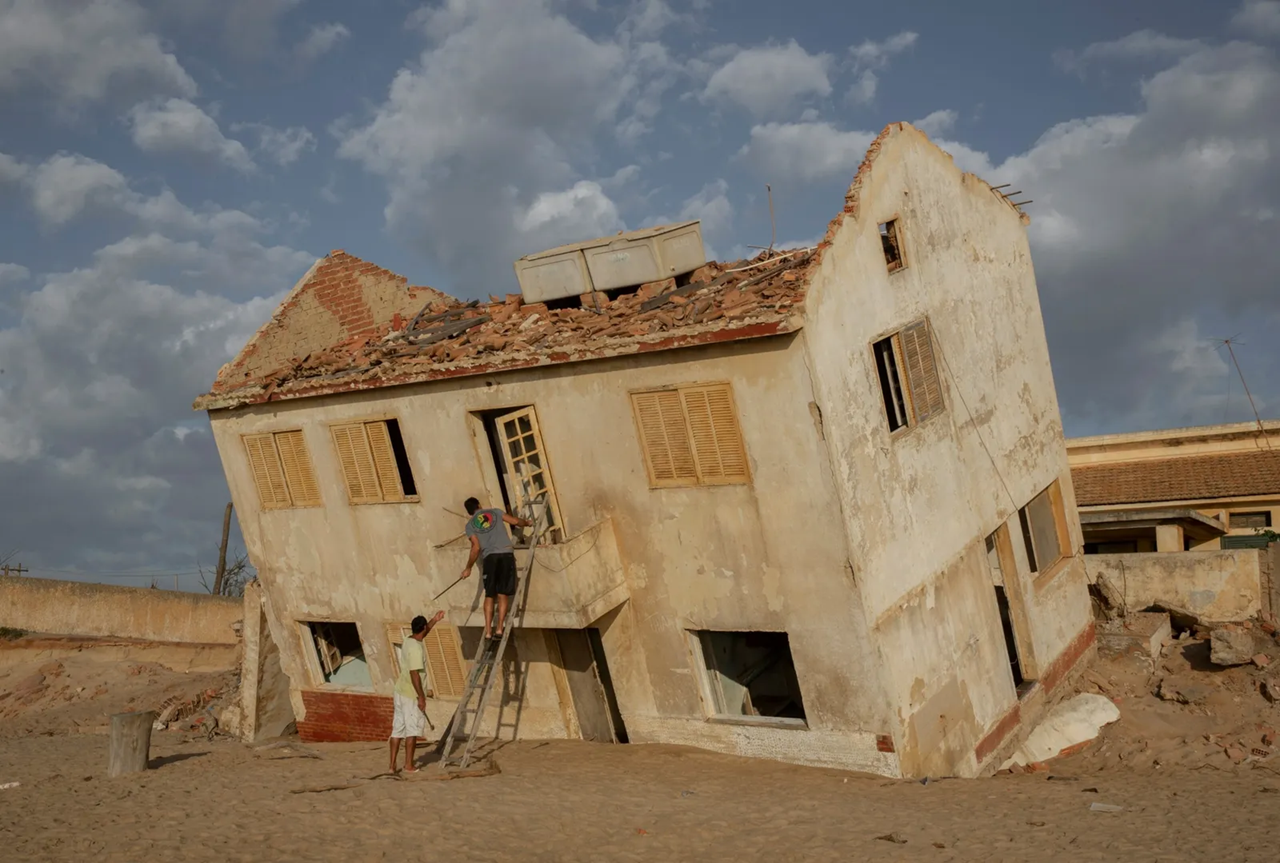
\includegraphics[width=\linewidth,height=0.59\textheight,keepaspectratio]{Atafona_2.png}
    \fonte{\textcite{briso_atafona_2021}.}
  \end{column}
  \begin{column}{0.48\textwidth}
    \centering
    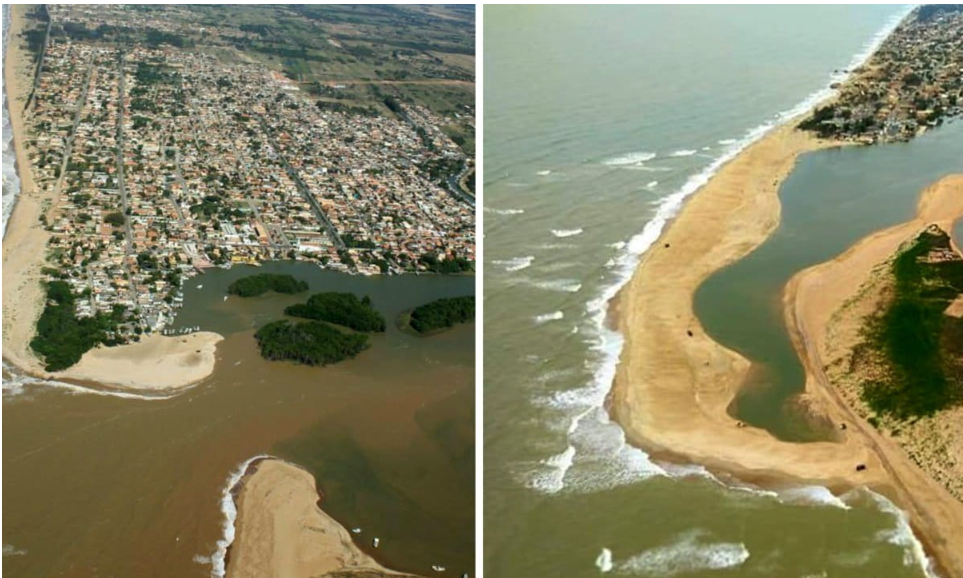
\includegraphics[width=\linewidth,height=0.59\textheight,keepaspectratio]{comparativo_02_19.png}
    \fonte{\textcite{briso_atafona_2021}.}
  \end{column}
\end{columns}
\vspace{0.5em}
\centering
\small Compreender a erosão costeira em Atafona a partir da caracterização da área e da análise integrada de informações cartográficas e oceanográficas.
\end{frame}

\section{Metodologia}
\begin{frame}{Metodologia}
\begin{columns}[T,onlytextwidth]
  \begin{column}{0.52\textwidth}
    \centering
    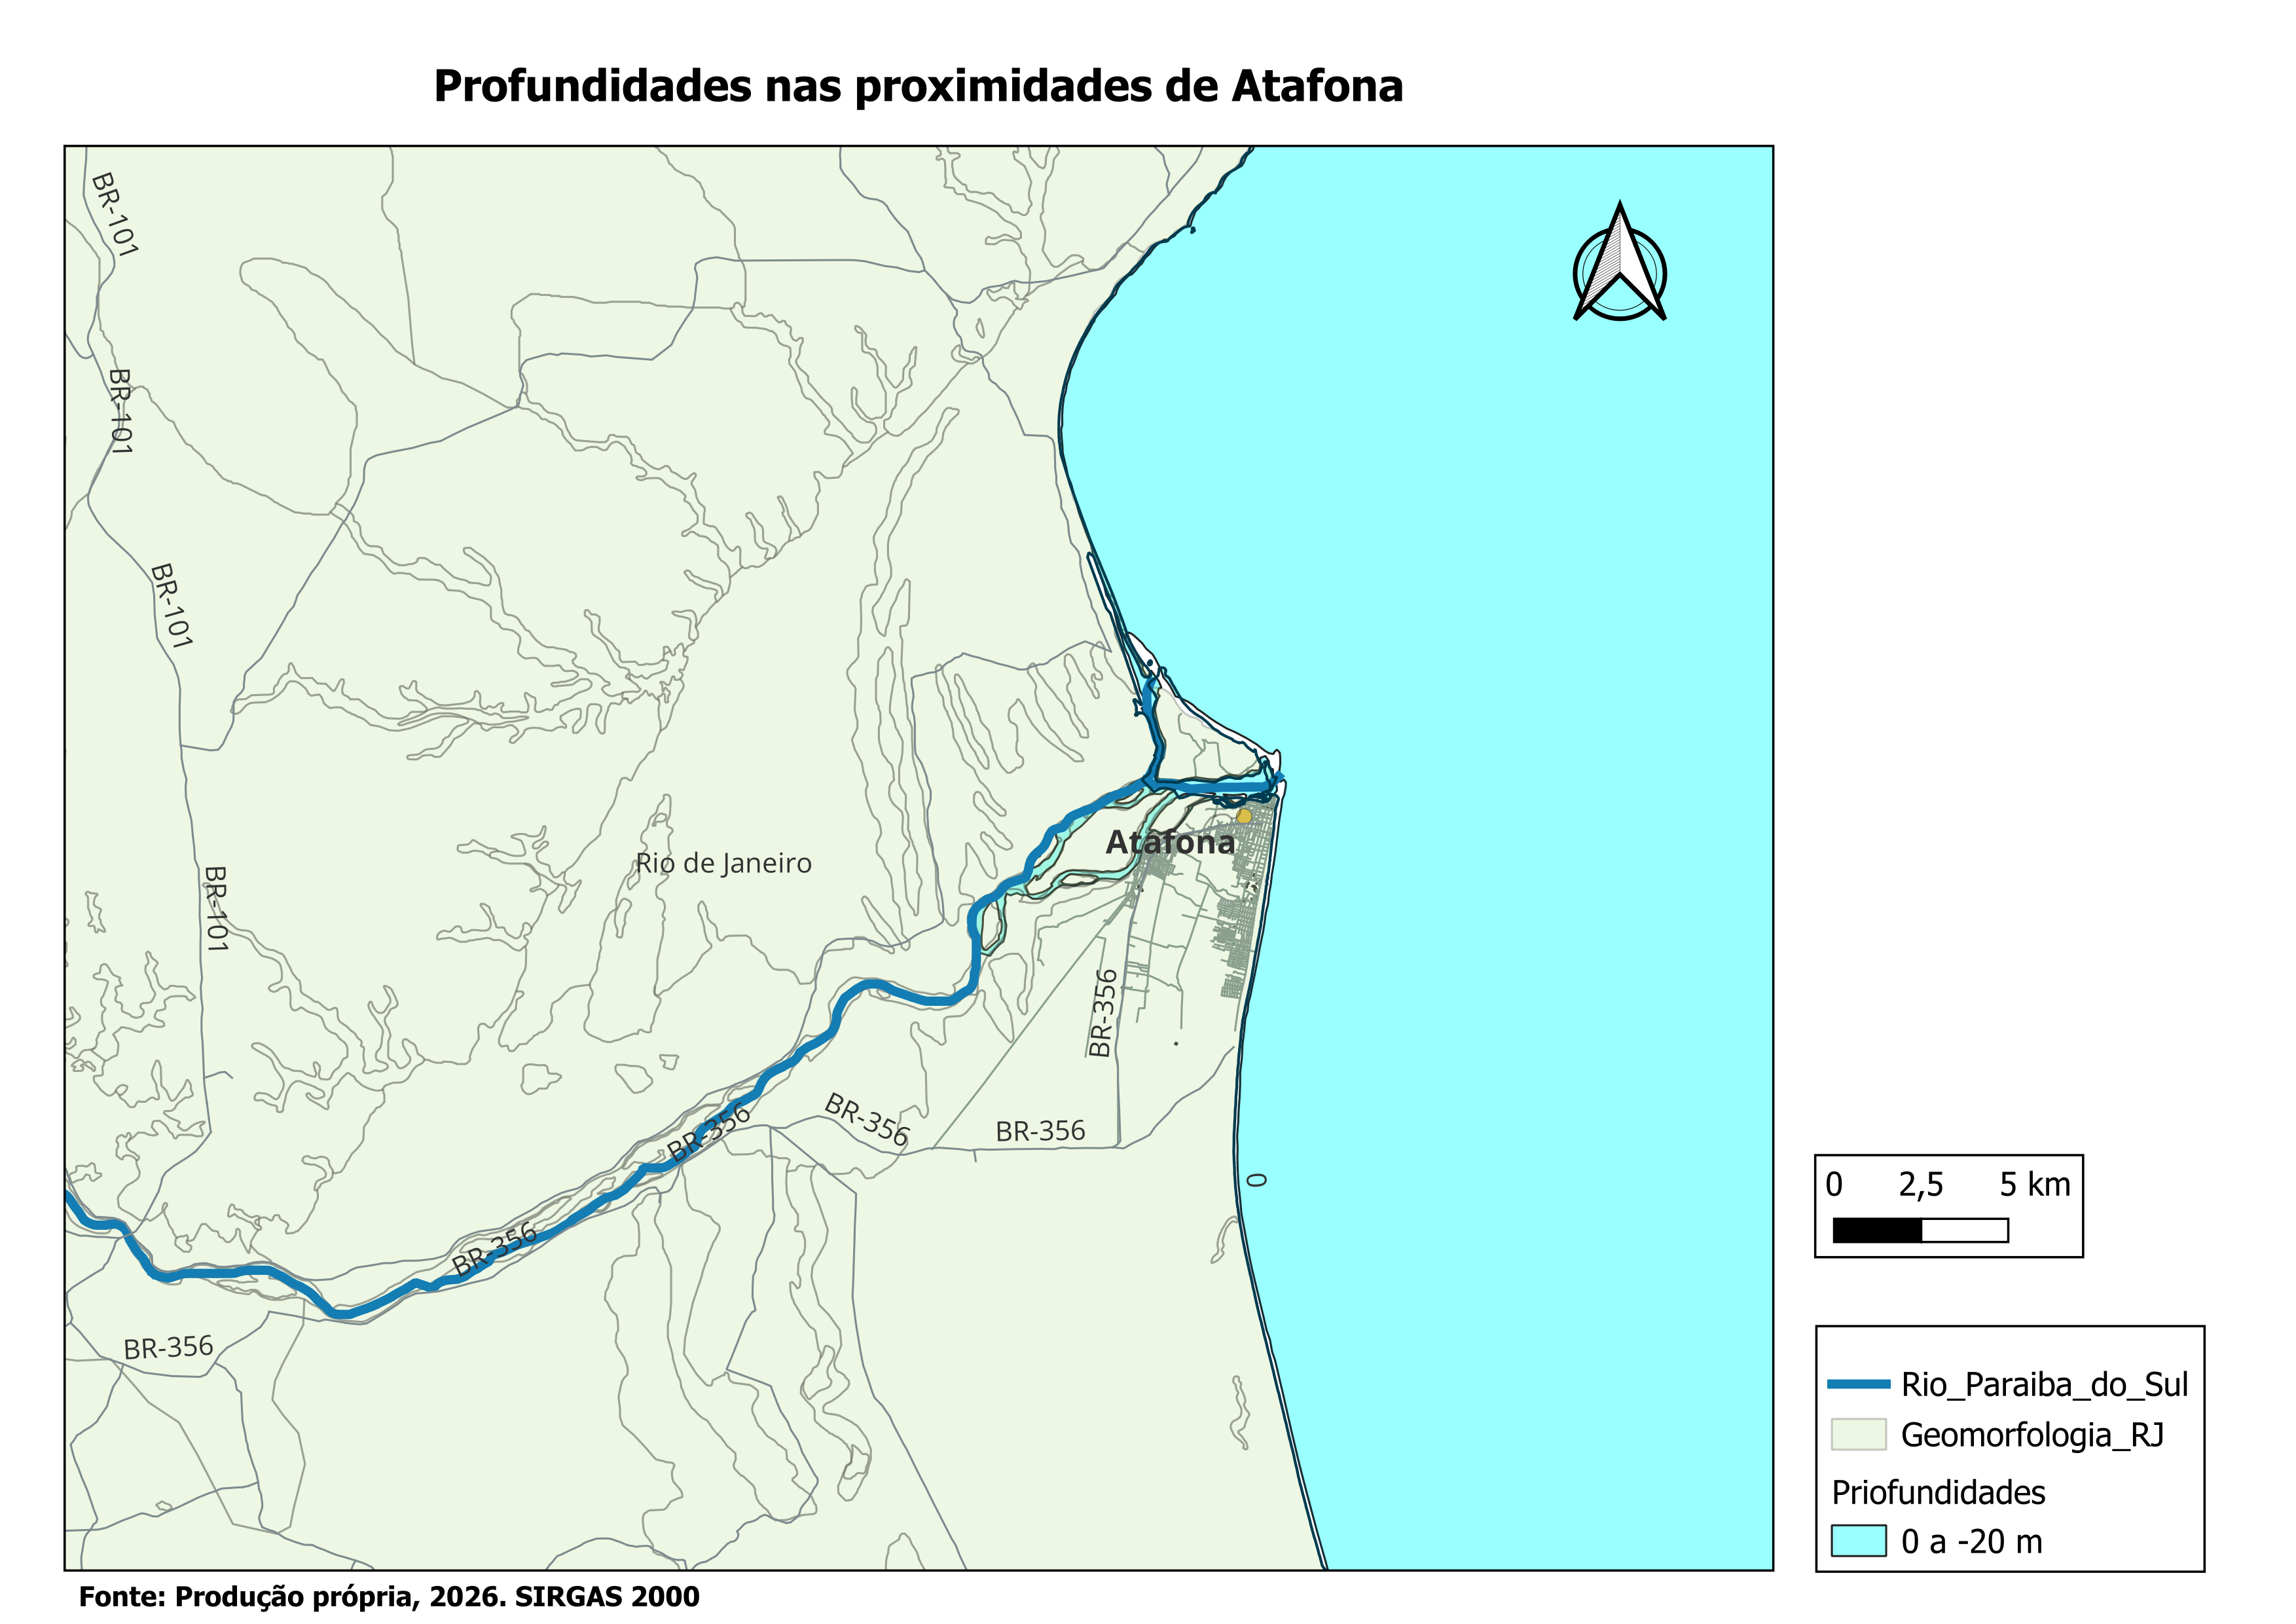
\includegraphics[width=0.95\linewidth,height=0.52\textheight,keepaspectratio]{batimetria_Atafona.png}
    %\fonte{material cartográfico do grupo.}
  \end{column}
  \begin{column}{0.44\textwidth}
    \centering
    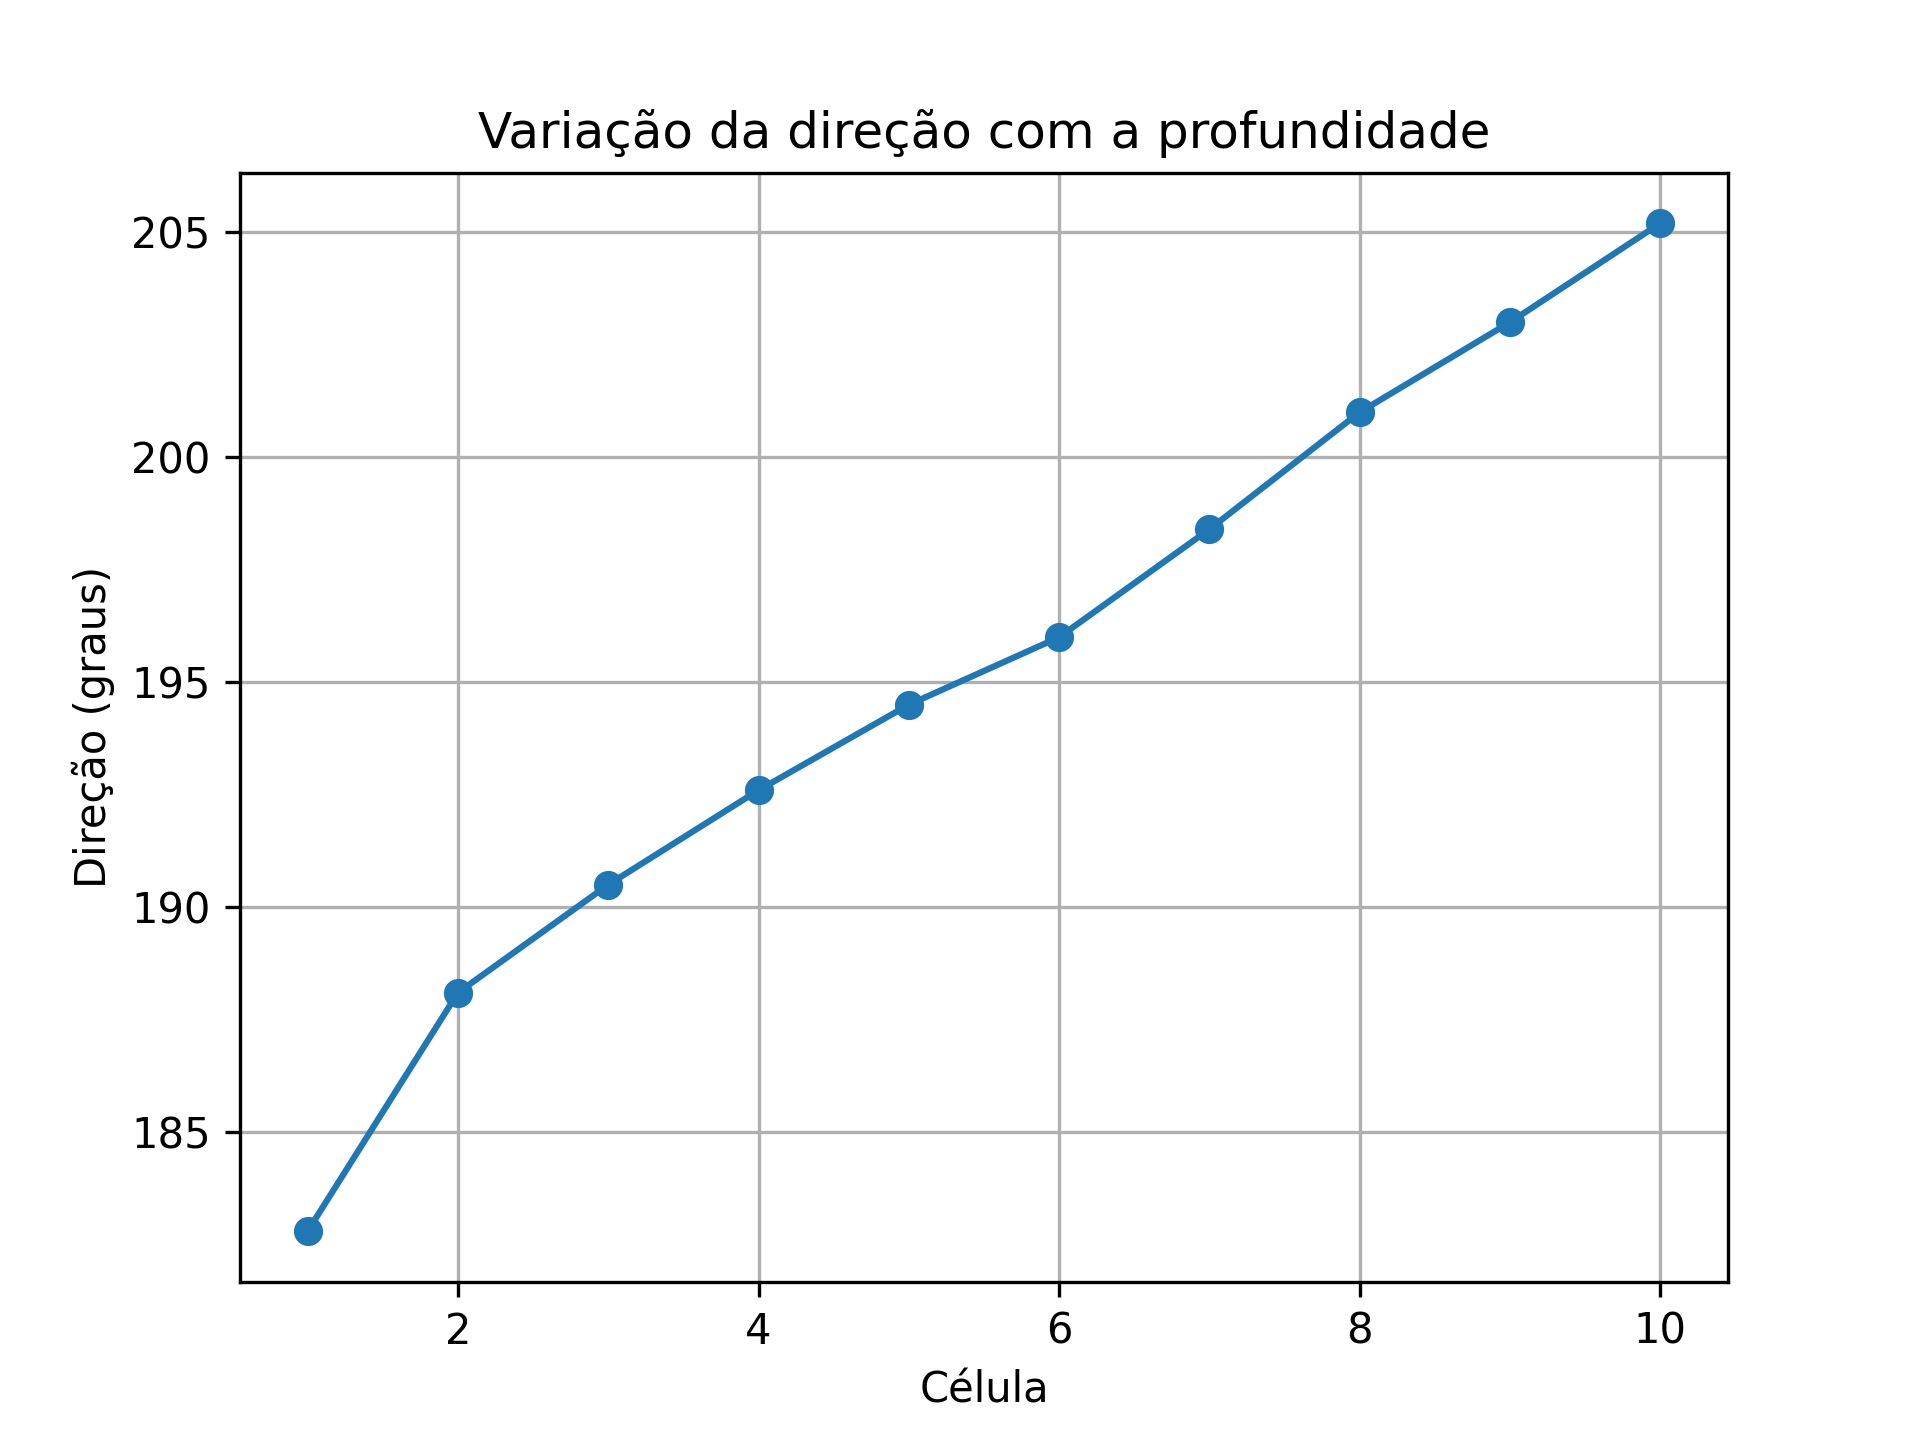
\includegraphics[width=0.98\linewidth,height=0.40\textheight,keepaspectratio]{direcao_cells.png}
    %\fonte{elaboração do grupo com dados do \textcite{simcosta_dados_2026}.}
    \vspace{0.4em}
    \begin{itemize}
      \item análise de mapas e imagens;
      \item comparação da linha de costa;
      \item interpretação de batimetria e correntes.
    \end{itemize}
  \end{column}
\end{columns}
\end{frame}

\section{Resultados}
\begin{frame}{Resultados: caracterização fisiográfica}
\begin{columns}[T,onlytextwidth]
  \begin{column}{0.63\textwidth}
    \centering
    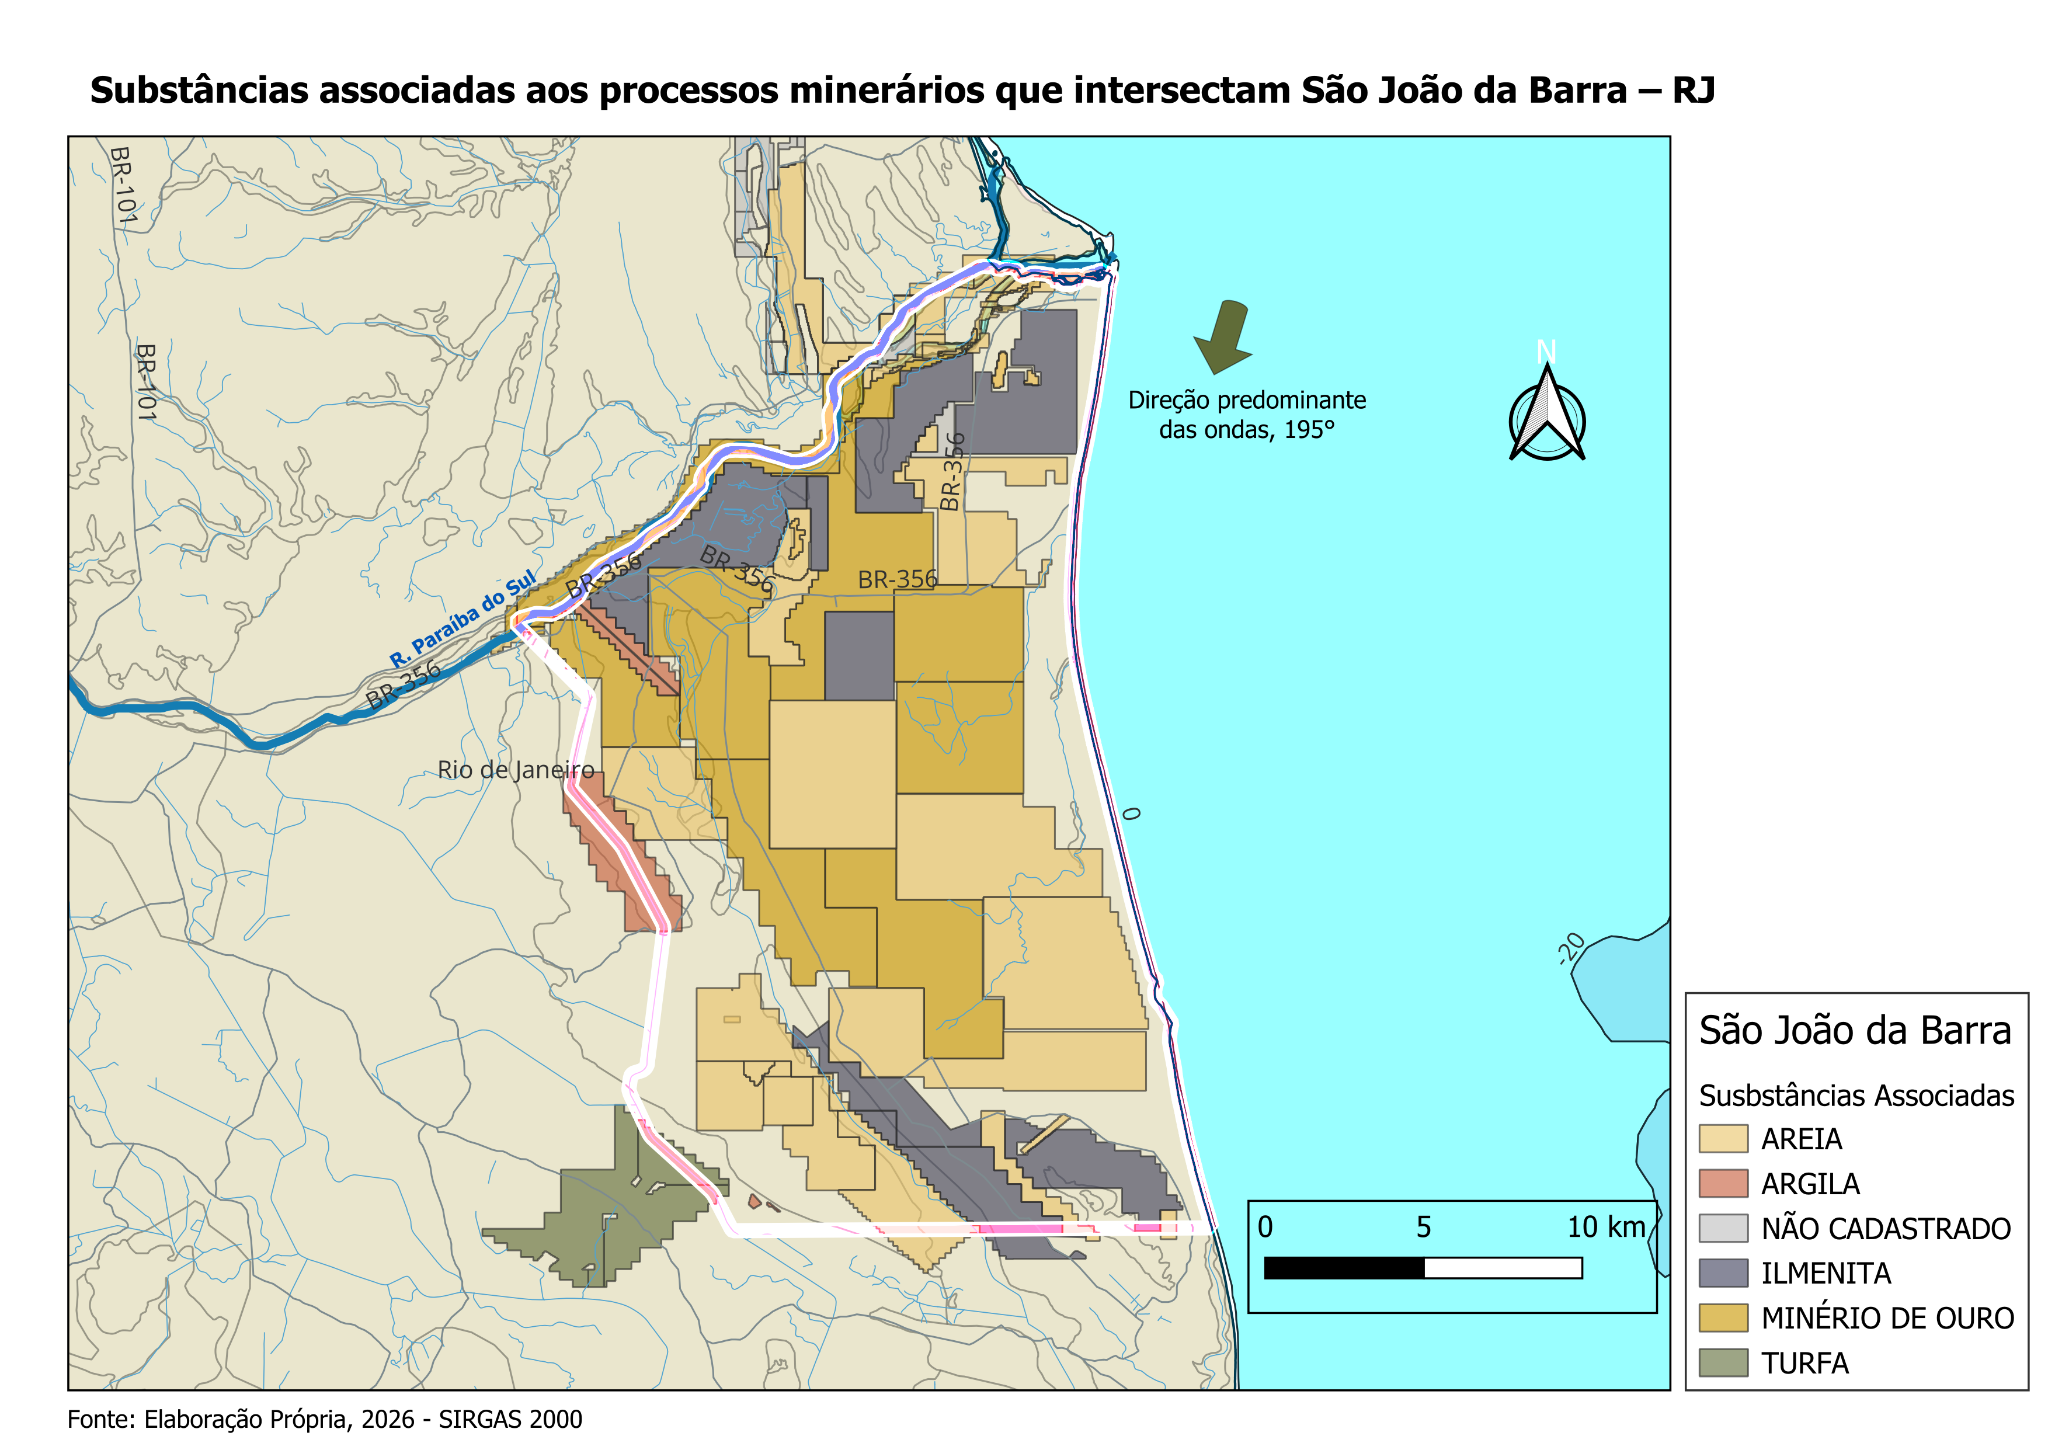
\includegraphics[width=\linewidth,height=0.70\textheight,keepaspectratio]{Mapa_Processos_Minerarios_SJB.png}
    %\fonte{material cartográfico do grupo.}
  \end{column}
  \begin{column}{0.33\textwidth}
    \vspace{1.5em}
    \begin{itemize}
      \item sistema deltaico sujeito a elevada mobilidade morfológica;
      \item relevo baixo e materiais pouco consolidados;
      \item linha de costa sensível a mudanças no balanço sedimentar.
    \end{itemize}
  \end{column}
\end{columns}
\end{frame}

\begin{frame}{Resultados: evolução da linha de costa}
\begin{columns}[T,onlytextwidth]
  \begin{column}{0.54\textwidth}
    \centering
    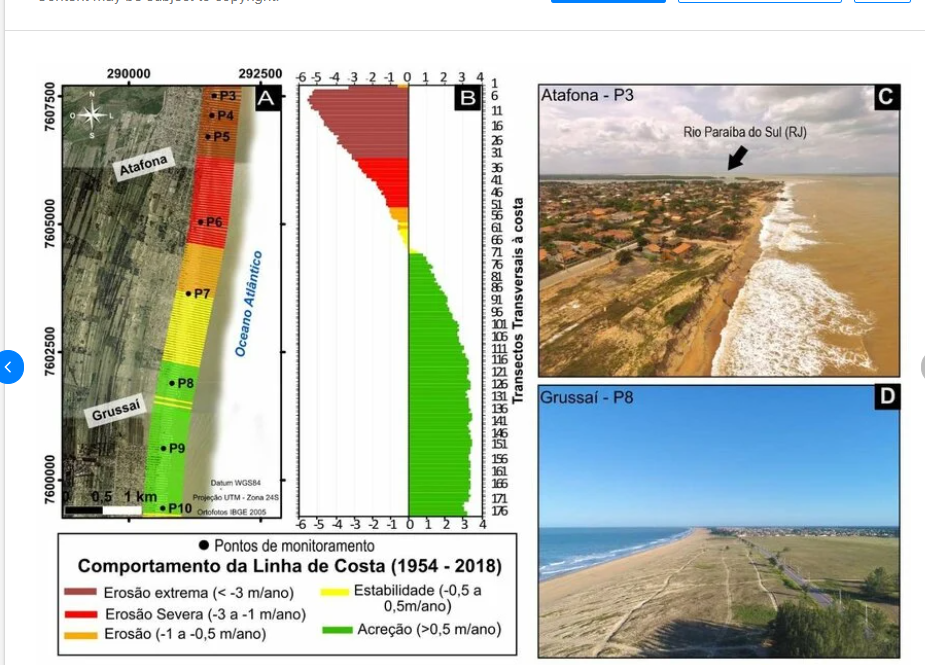
\includegraphics[width=\linewidth,height=0.60\textheight,keepaspectratio]{atafona_grussai.png}
    \fonte{\textcite{machado2024_dinamica_linha_costa_paraiba_sul}.}
  \end{column}
  \begin{column}{0.42\textwidth}
    \centering
    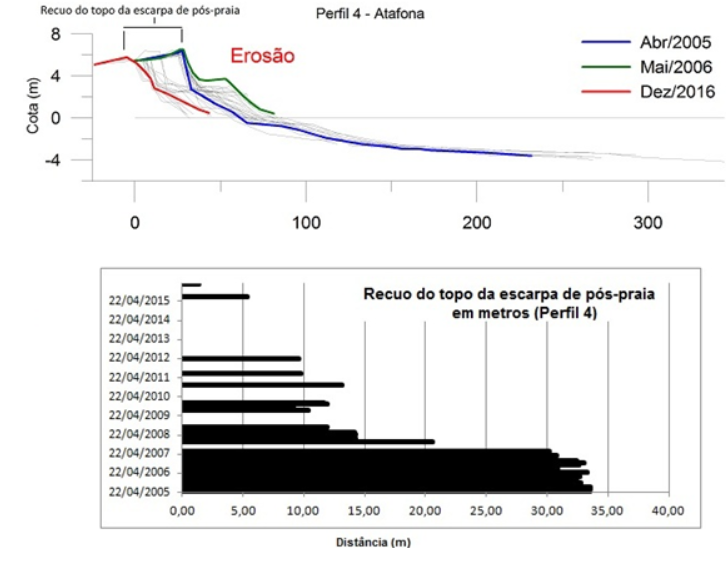
\includegraphics[width=\linewidth,height=0.51\textheight,keepaspectratio]{avanço_erosão.png}
    \fonte{\textcite{mello2018_erosao_atafona}.}
  \end{column}
\end{columns}
\vspace{0.25em}
\centering
\small Os registros indicam recuo expressivo em Atafona e comportamento espacial distinto em trechos próximos.
\end{frame}

\begin{frame}{Resultados: batimetria}
\begin{columns}[T,onlytextwidth]
  \begin{column}{0.66\textwidth}
    \centering
    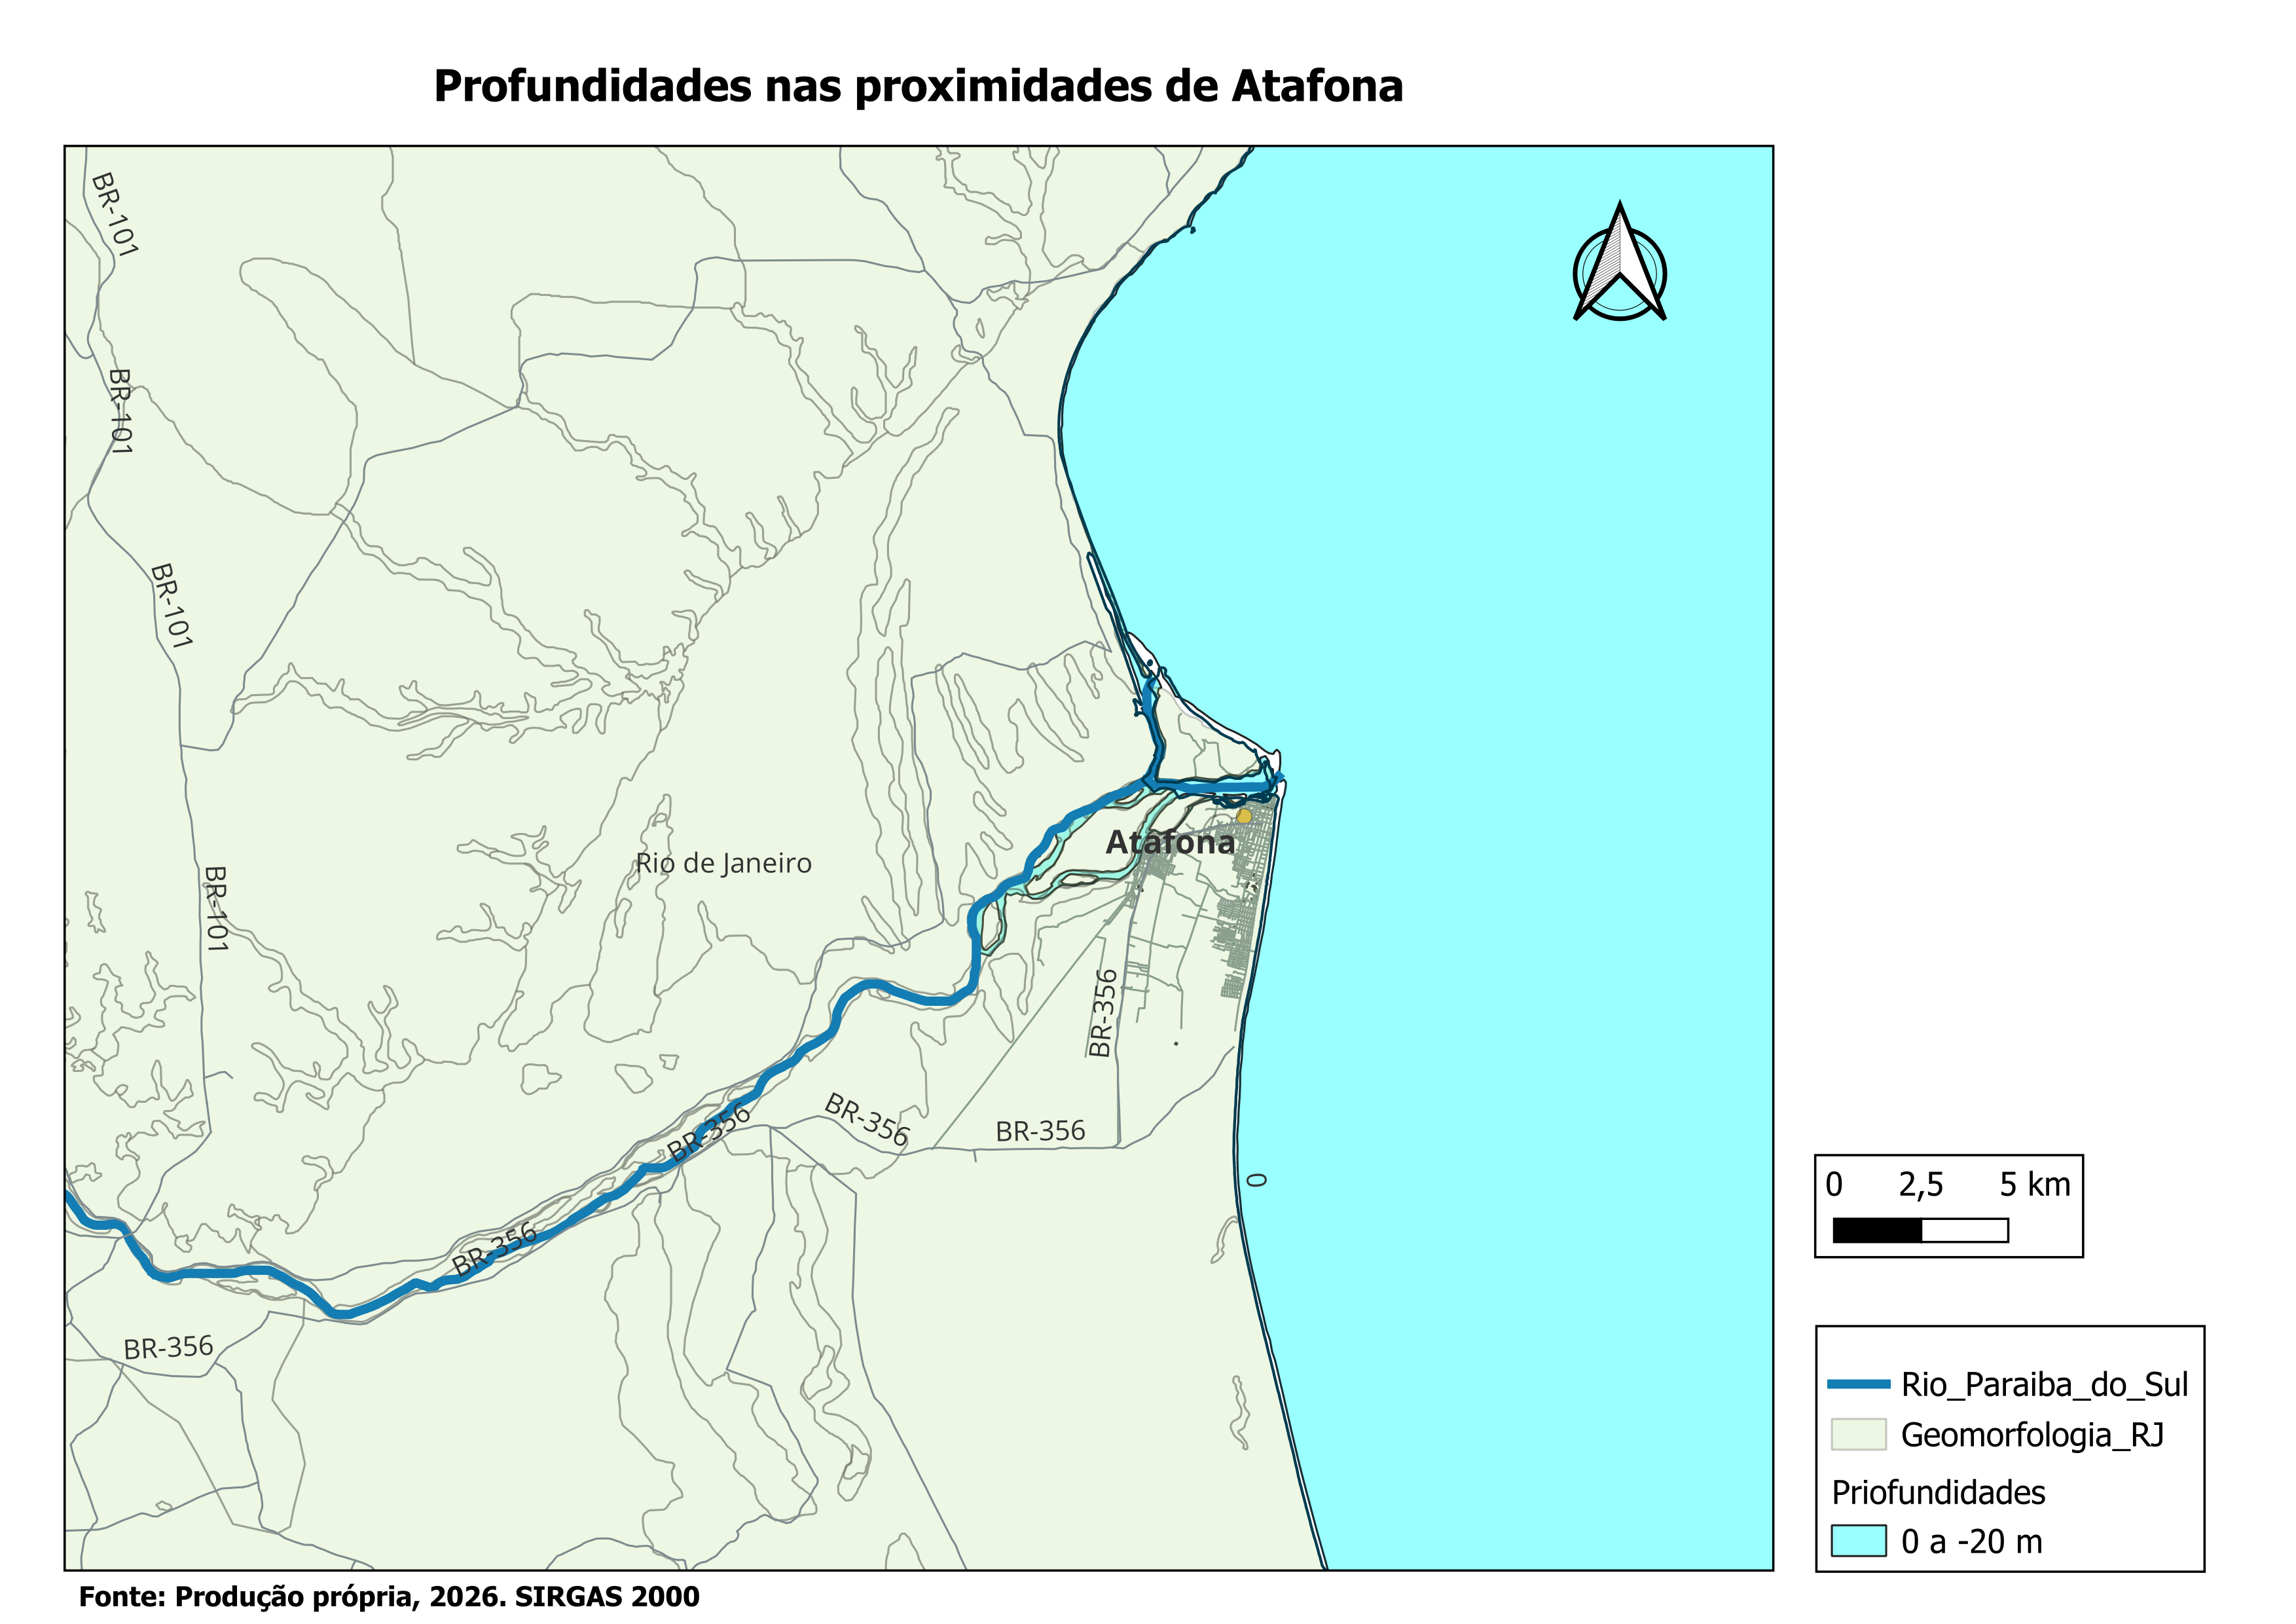
\includegraphics[width=\linewidth,height=0.71\textheight,keepaspectratio]{batimetria_Atafona.png}
    %\fonte{material cartográfico do grupo.}
  \end{column}
  \begin{column}{0.30\textwidth}
    \vspace{2.2em}
    \begin{itemize}
      \item plataforma interna de baixa declividade;
      \item variações do relevo submarino próximas à foz;
      \item controle da propagação de ondas e do transporte sedimentar.
    \end{itemize}
  \end{column}
\end{columns}
\end{frame}

\begin{frame}{Resultados: aspectos oceanográficos}
\begin{columns}[T,onlytextwidth]
  \begin{column}{0.50\textwidth}
    \centering
    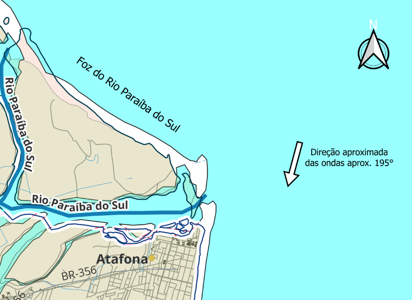
\includegraphics[width=\linewidth,height=0.62\textheight,keepaspectratio]{Aprox_195graus.png}
    \fonte{elaboração do grupo com dados do \textcite{simcosta_dados_2026}.}
  \end{column}
  \begin{column}{0.46\textwidth}
    \centering
    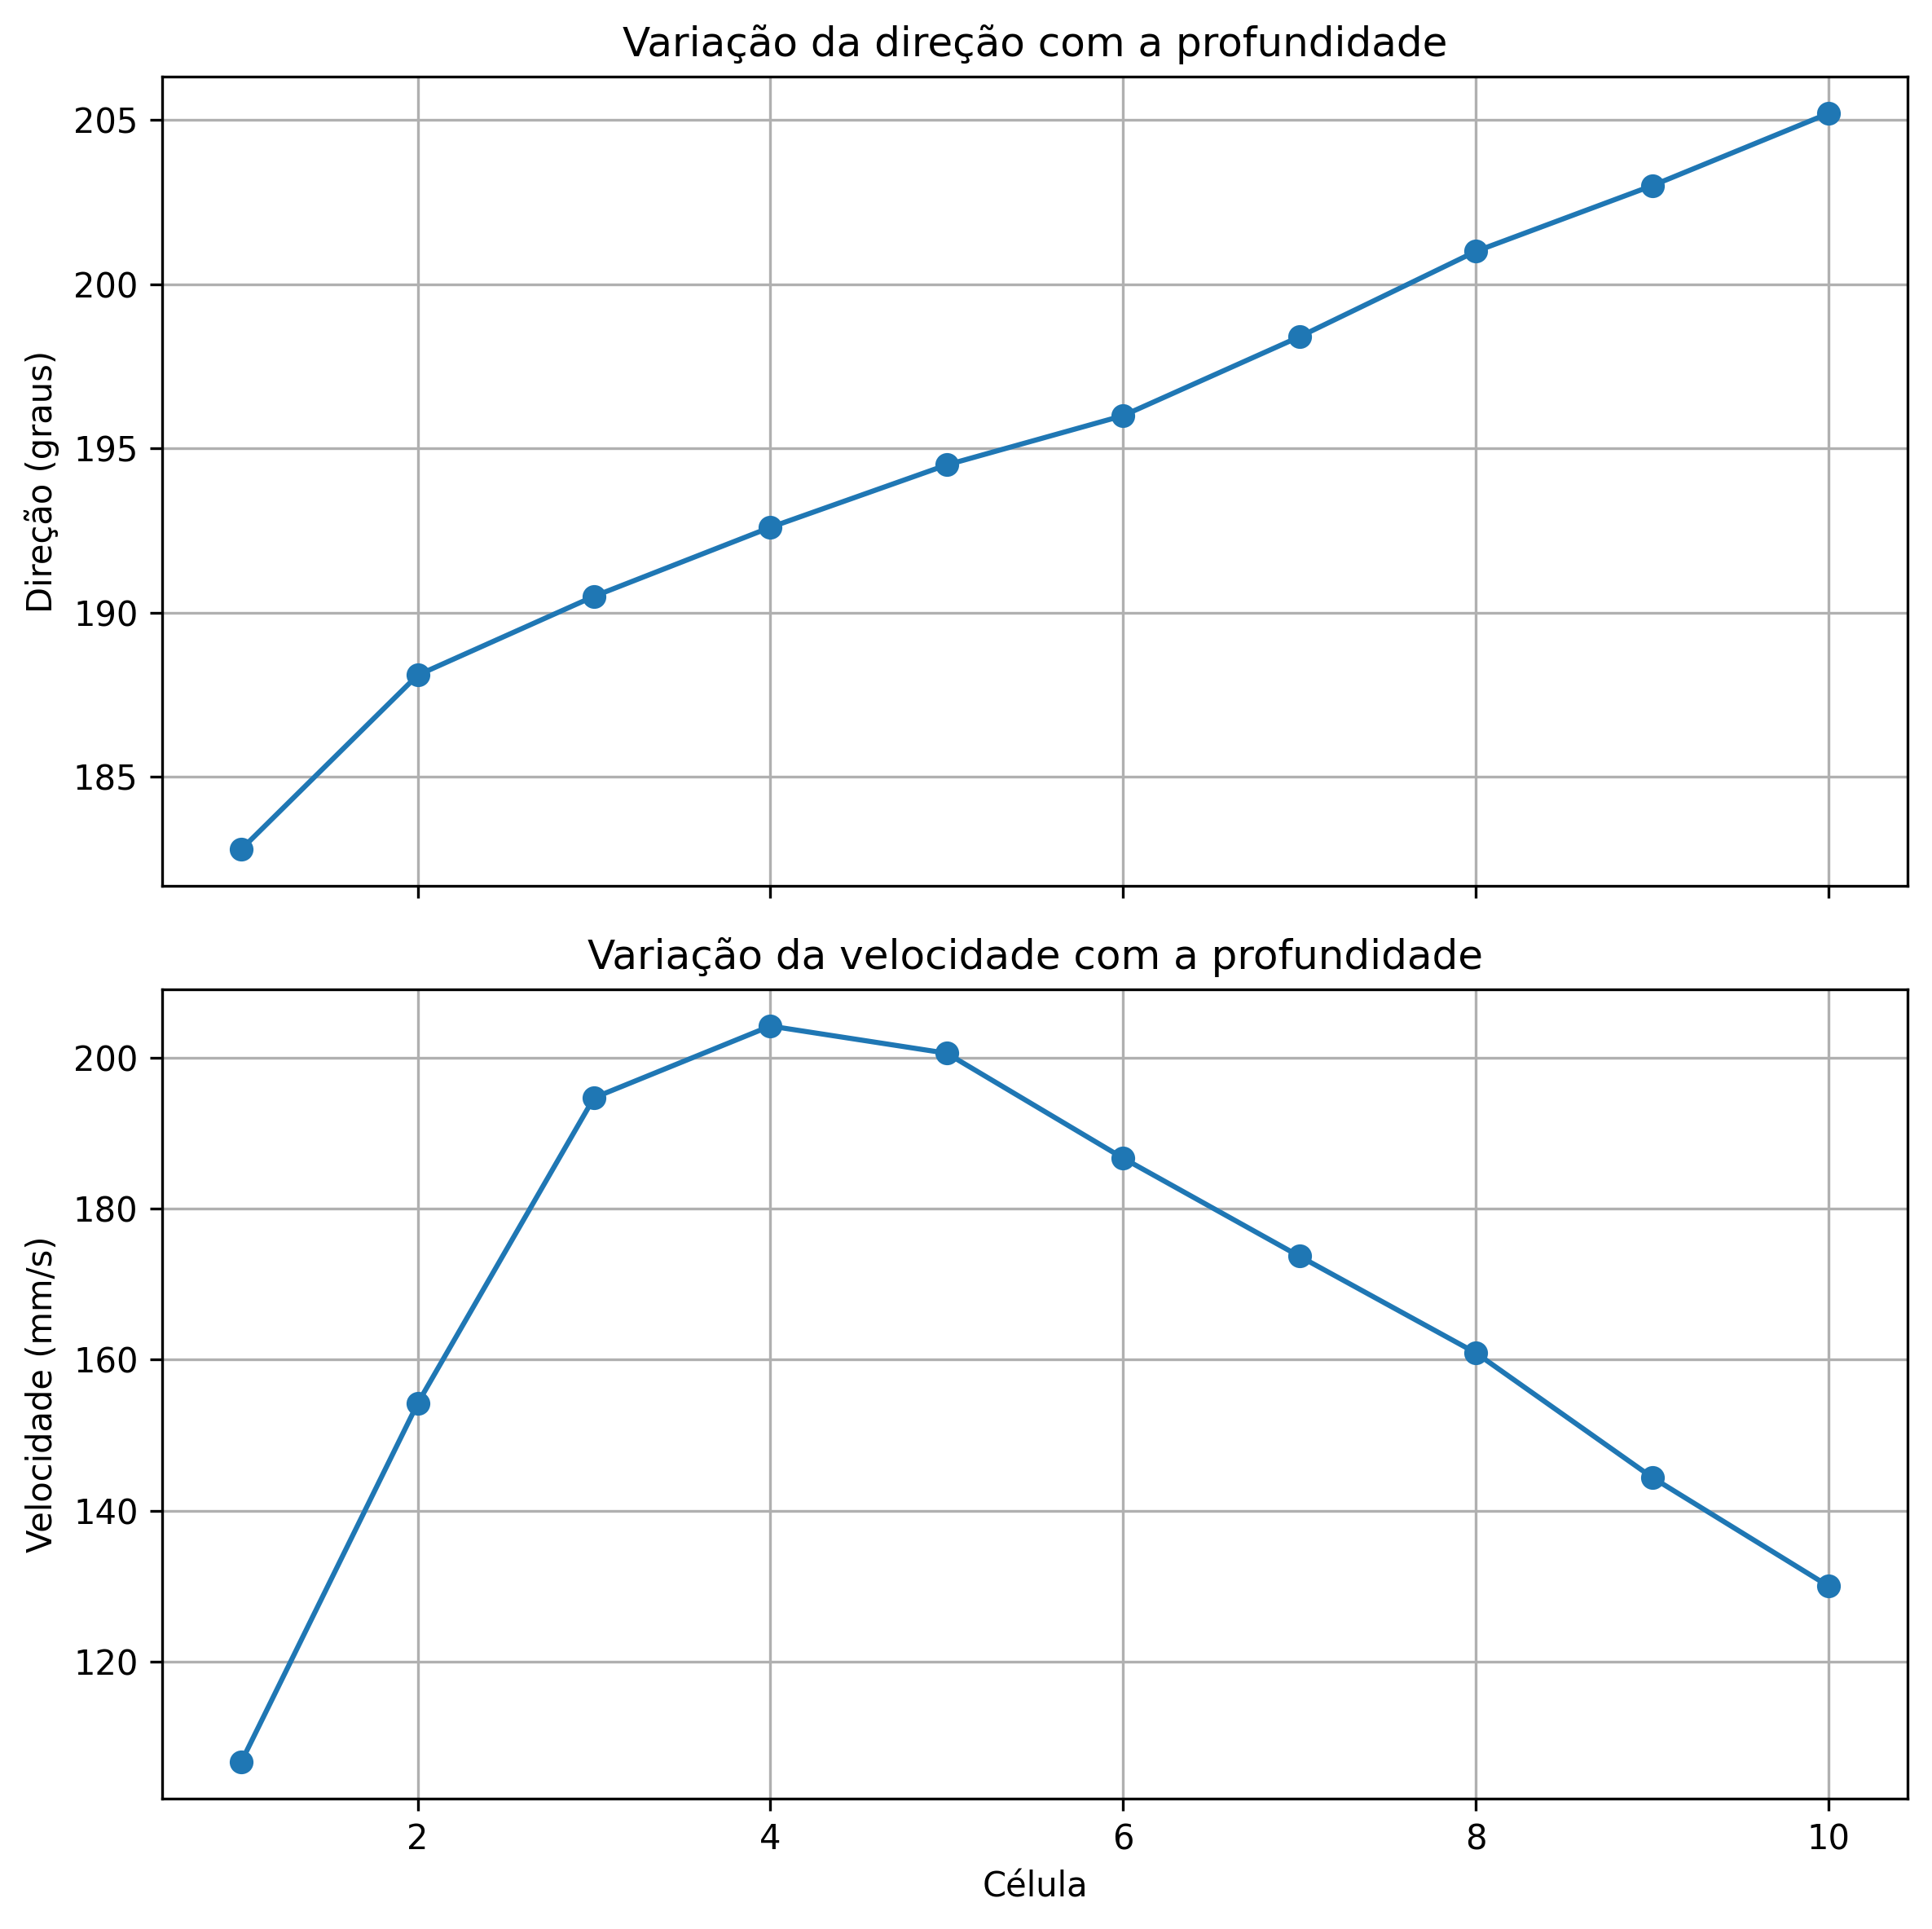
\includegraphics[width=\linewidth,height=0.43\textheight,keepaspectratio]{direcao_velocidade_cells.png}
    \vspace{0.4em}
    \small
    \begin{itemize}
      \item vetor de referência: \(0{,}165\ \mathrm{m\,s^{-1}}\), azimute aproximado de \(195^\circ\);
      \item dados da estação SiMCosta de Linhares;
      \item uso exploratório, sujeito à validação local em Atafona.
    \end{itemize}
  \end{column}
\end{columns}
\end{frame}

\begin{frame}{Resultados: dinâmica costeira}
\begin{columns}[T,onlytextwidth]
  \begin{column}{0.57\textwidth}
    \centering
    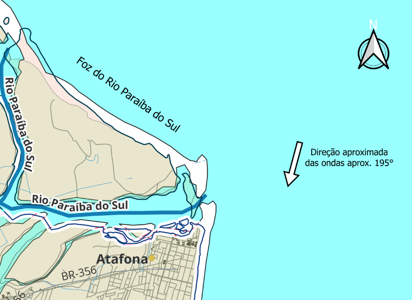
\includegraphics[width=\linewidth,height=0.69\textheight,keepaspectratio]{Aprox_195graus.png}
    \fonte{material cartográfico do grupo e \textcite{simcosta_dados_2026}.}
  \end{column}
  \begin{column}{0.39\textwidth}
    \vspace{1.0em}
    \begin{itemize}
      \item a foz integra processos fluviais e marinhos;
      \item alterações no aporte sedimentar modificam esse equilíbrio;
      \item ondas e correntes redistribuem os sedimentos ao longo da costa;
      \item os dados regionais não substituem medições locais.
    \end{itemize}
  \end{column}
\end{columns}
\end{frame}

\section{Conclusão e discussões}
\begin{frame}{Conclusão e discussões}
\begin{columns}[T,onlytextwidth]
  \begin{column}{0.48\textwidth}
    \centering
    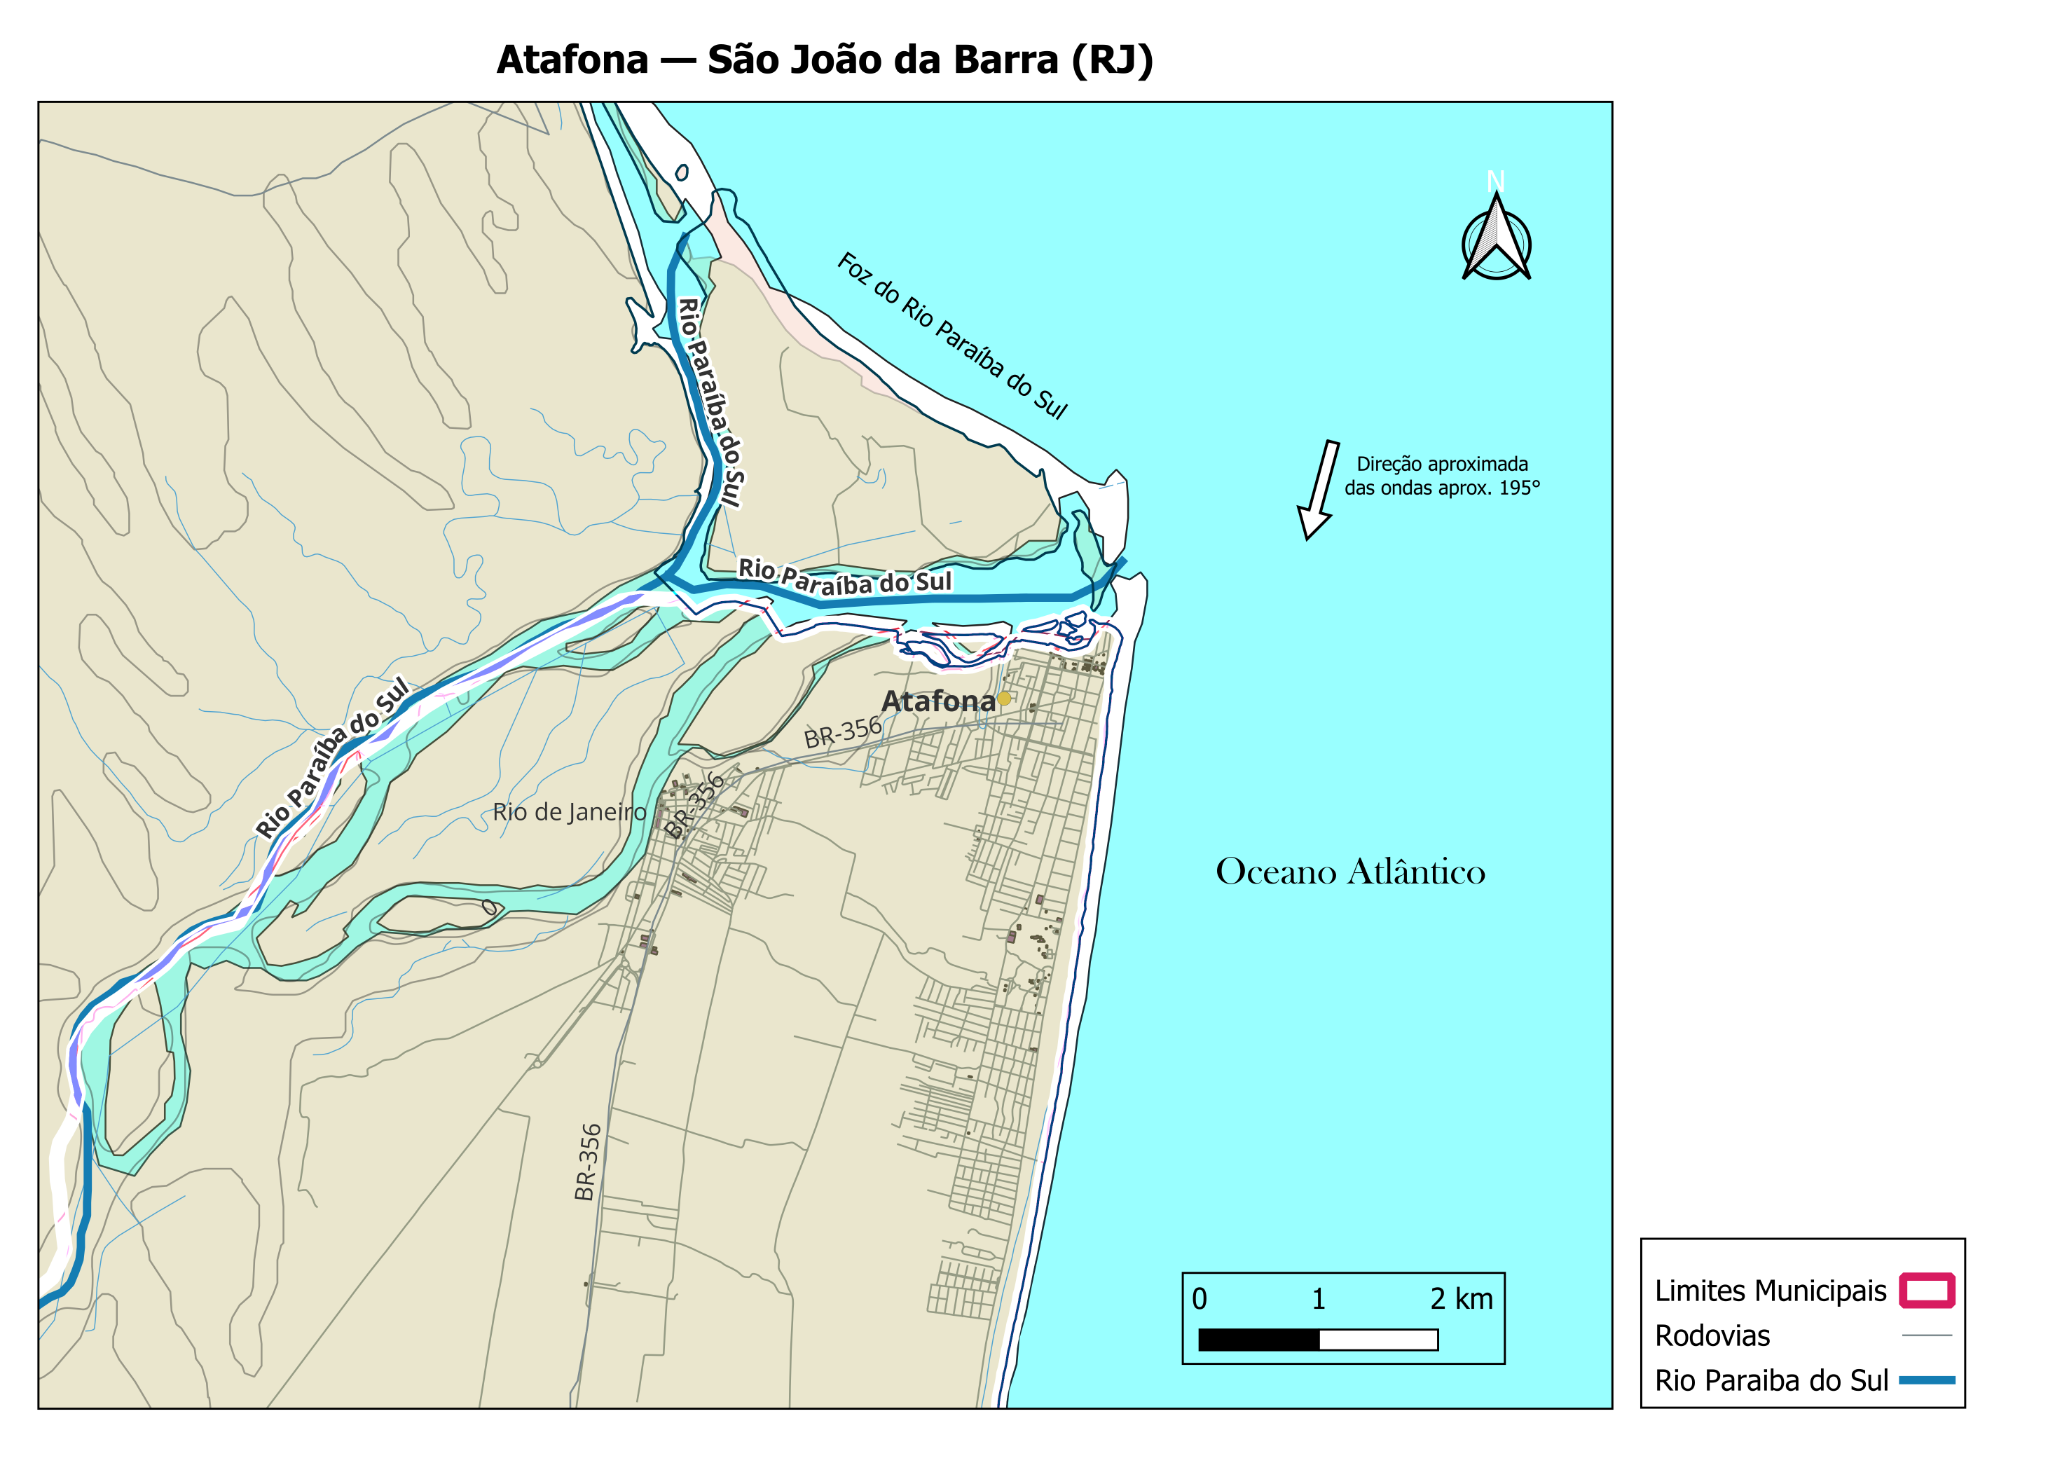
\includegraphics[width=\linewidth,height=0.64\textheight,keepaspectratio]{Atafona.png}
    \fonte{material cartográfico do grupo.}
  \end{column}
  \begin{column}{0.48\textwidth}
    \vspace{1.2em}
    \begin{itemize}
      \item Atafona apresenta erosão costeira intensa e persistente.
      \item A configuração deltaica aumenta a sensibilidade às mudanças do balanço sedimentar.
      \item A interpretação exige integrar descarga fluvial, batimetria, ondas e correntes.
      \item A ausência de medições locais limita conclusões sobre a circulação junto à foz.
    \end{itemize}
  \end{column}
\end{columns}
\end{frame}

\section{Recomendações para o futuro}
\begin{frame}{Recomendações: alternativas de proteção costeira}
  \centering
  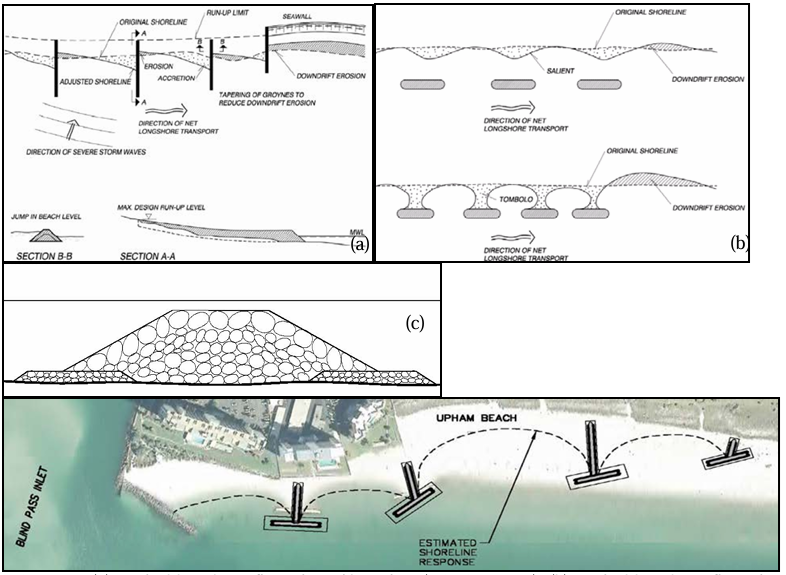
\includegraphics[width=0.93\linewidth,height=0.69\textheight,keepaspectratio]{configs.png}
  \fonte{\textcite{asbpa2011_erosion_control_structures}.}
  \vspace{0.3em}
  \small Espigões e quebra-mares modificam o campo de ondas e a redistribuição dos sedimentos. A escolha depende da resposta esperada da linha de costa.
\end{frame}

\begin{frame}{Recomendações: estudos necessários em Atafona}
\begin{columns}[T,onlytextwidth]
  \begin{column}{0.48\textwidth}
    \centering
    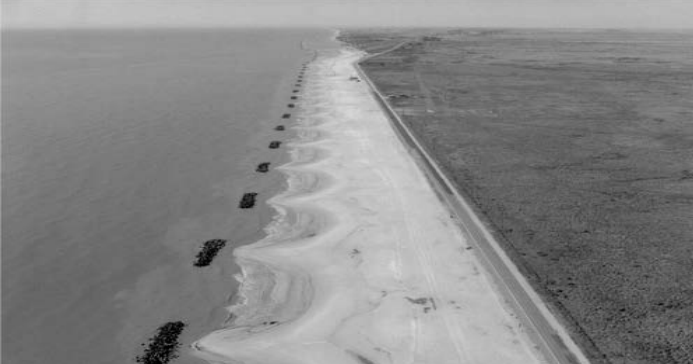
\includegraphics[width=\linewidth,height=0.42\textheight,keepaspectratio]{Holly_beach.png}
    \fonte{\textcite{asbpa2011_erosion_control_structures}.}
    \vspace{0.4em}
    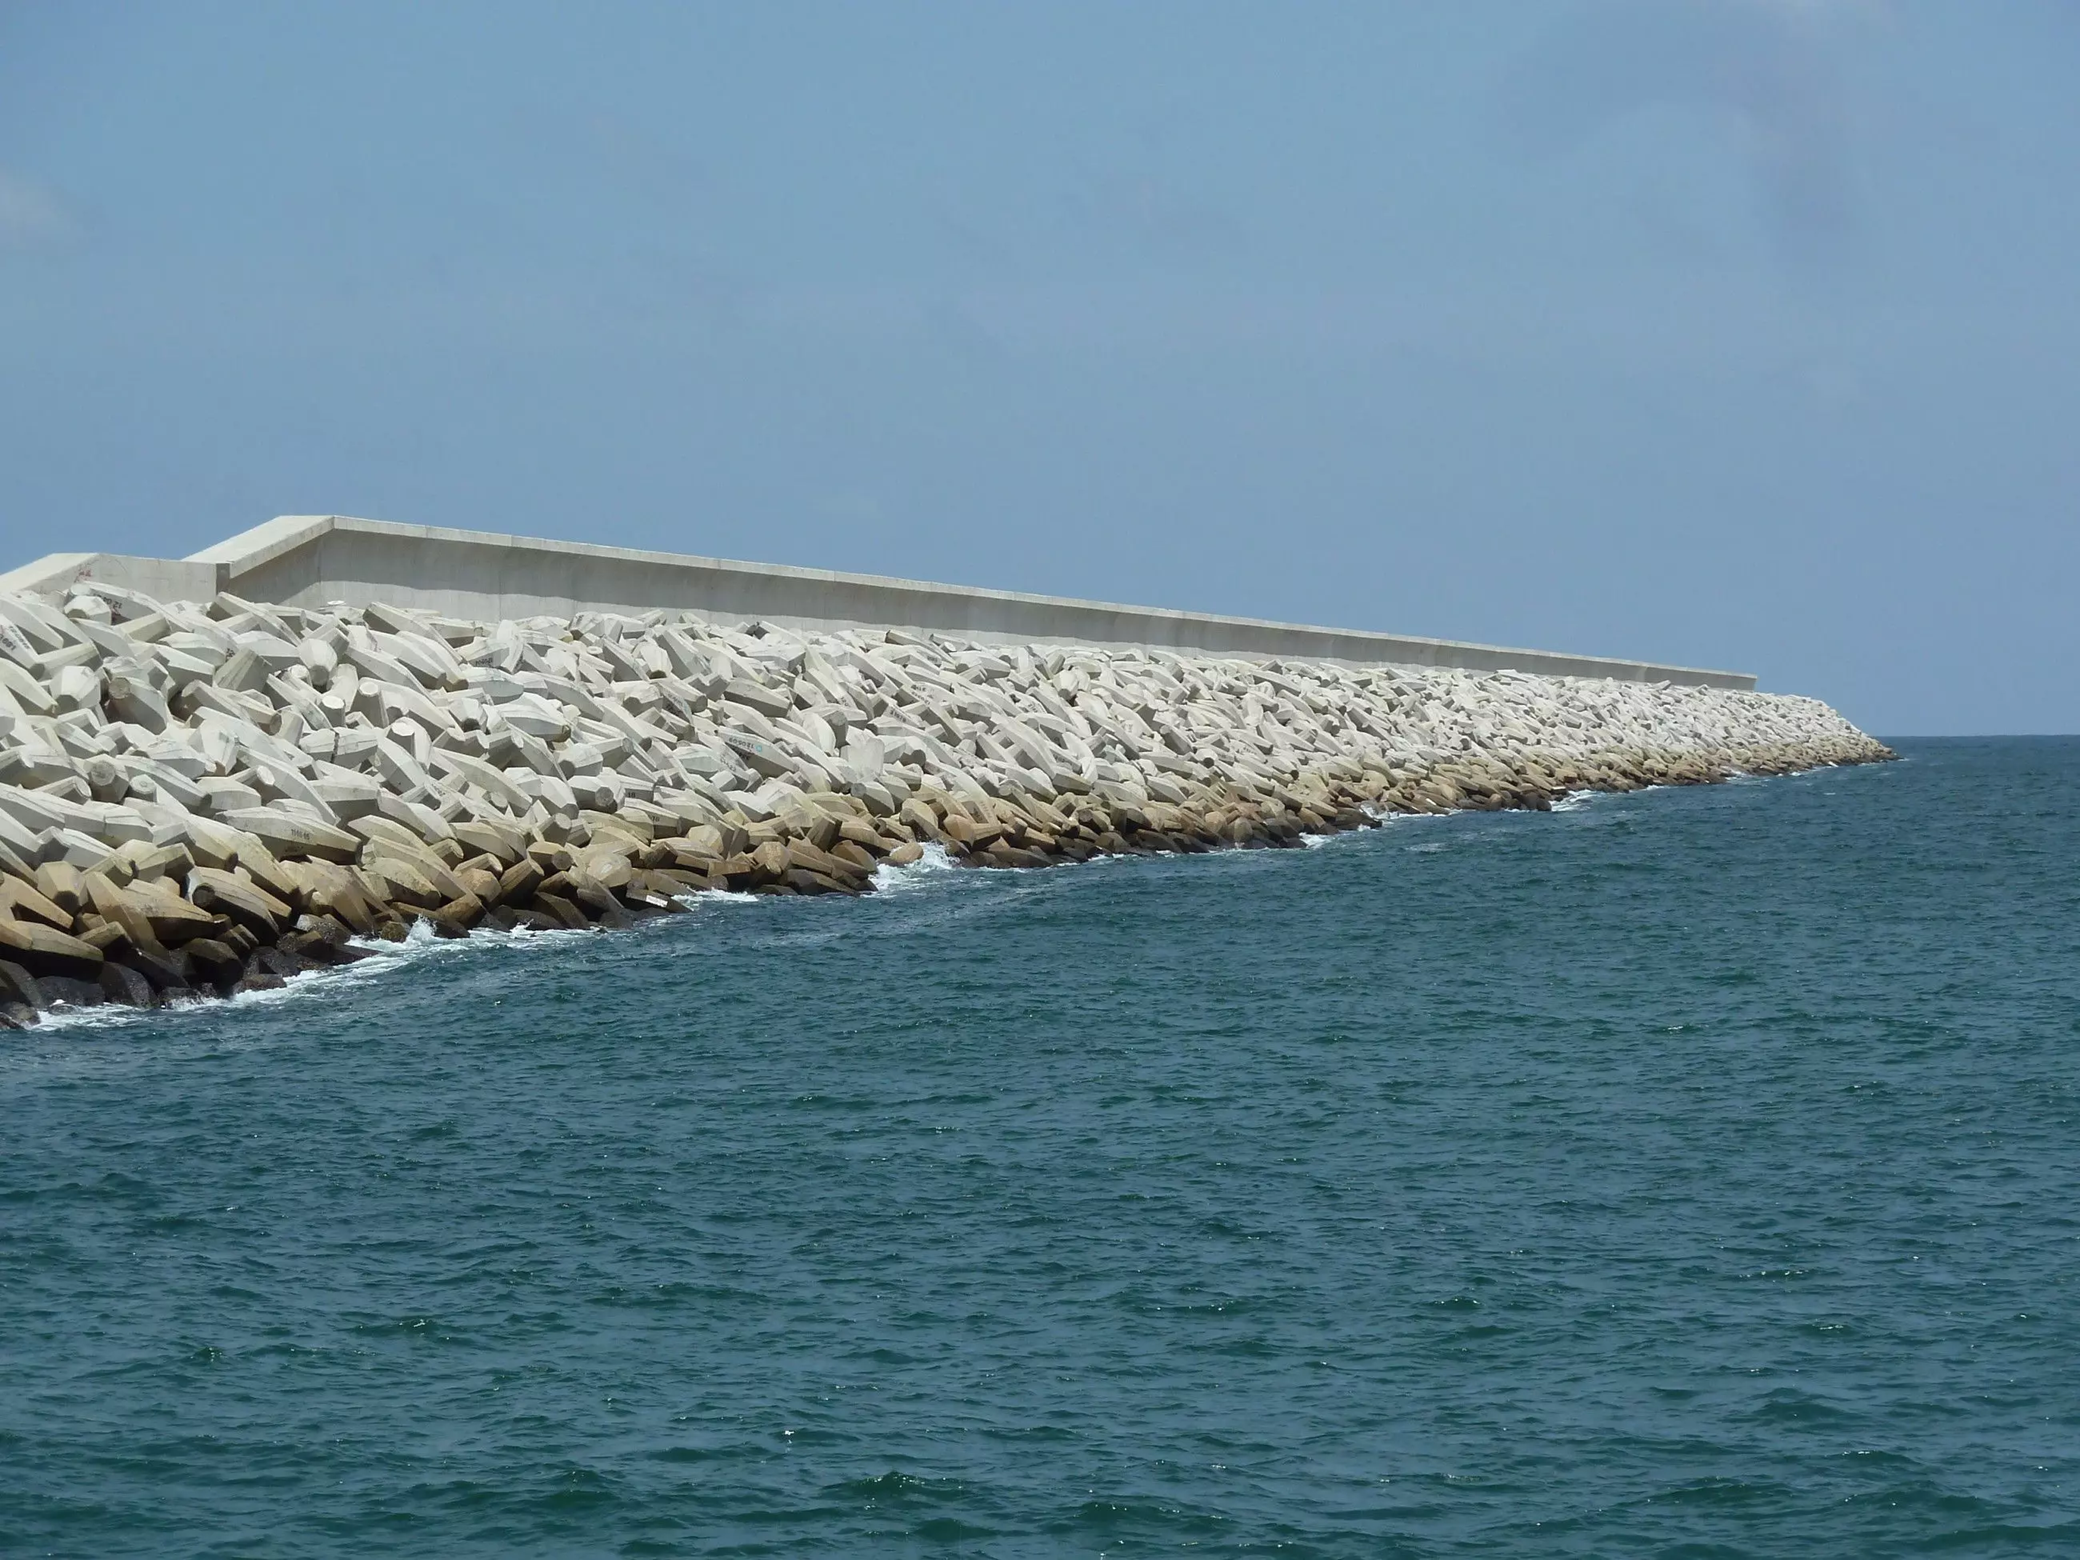
\includegraphics[width=\linewidth,height=0.27\textheight,keepaspectratio]{Core-loc_break_water.png}
    \fonte{\textcite{coreloc_imagem}.}
  \end{column}
  \begin{column}{0.48\textwidth}
    \vspace{1.4em}
    \begin{itemize}
      \item obter séries locais de ondas, correntes e transporte sedimentar;
      \item modelar diferentes configurações e cenários de intervenção;
      \item avaliar efeitos sobre praias e comunidades adjacentes;
      \item implantar monitoramento antes, durante e depois de qualquer obra.
    \end{itemize}
    \vspace{0.7em}
    \small Estruturas costeiras constituem alternativas de estudo, e não uma solução previamente definida para Atafona.
  \end{column}
\end{columns}
\end{frame}

\begin{frame}{Agradecimentos}
  \centering
  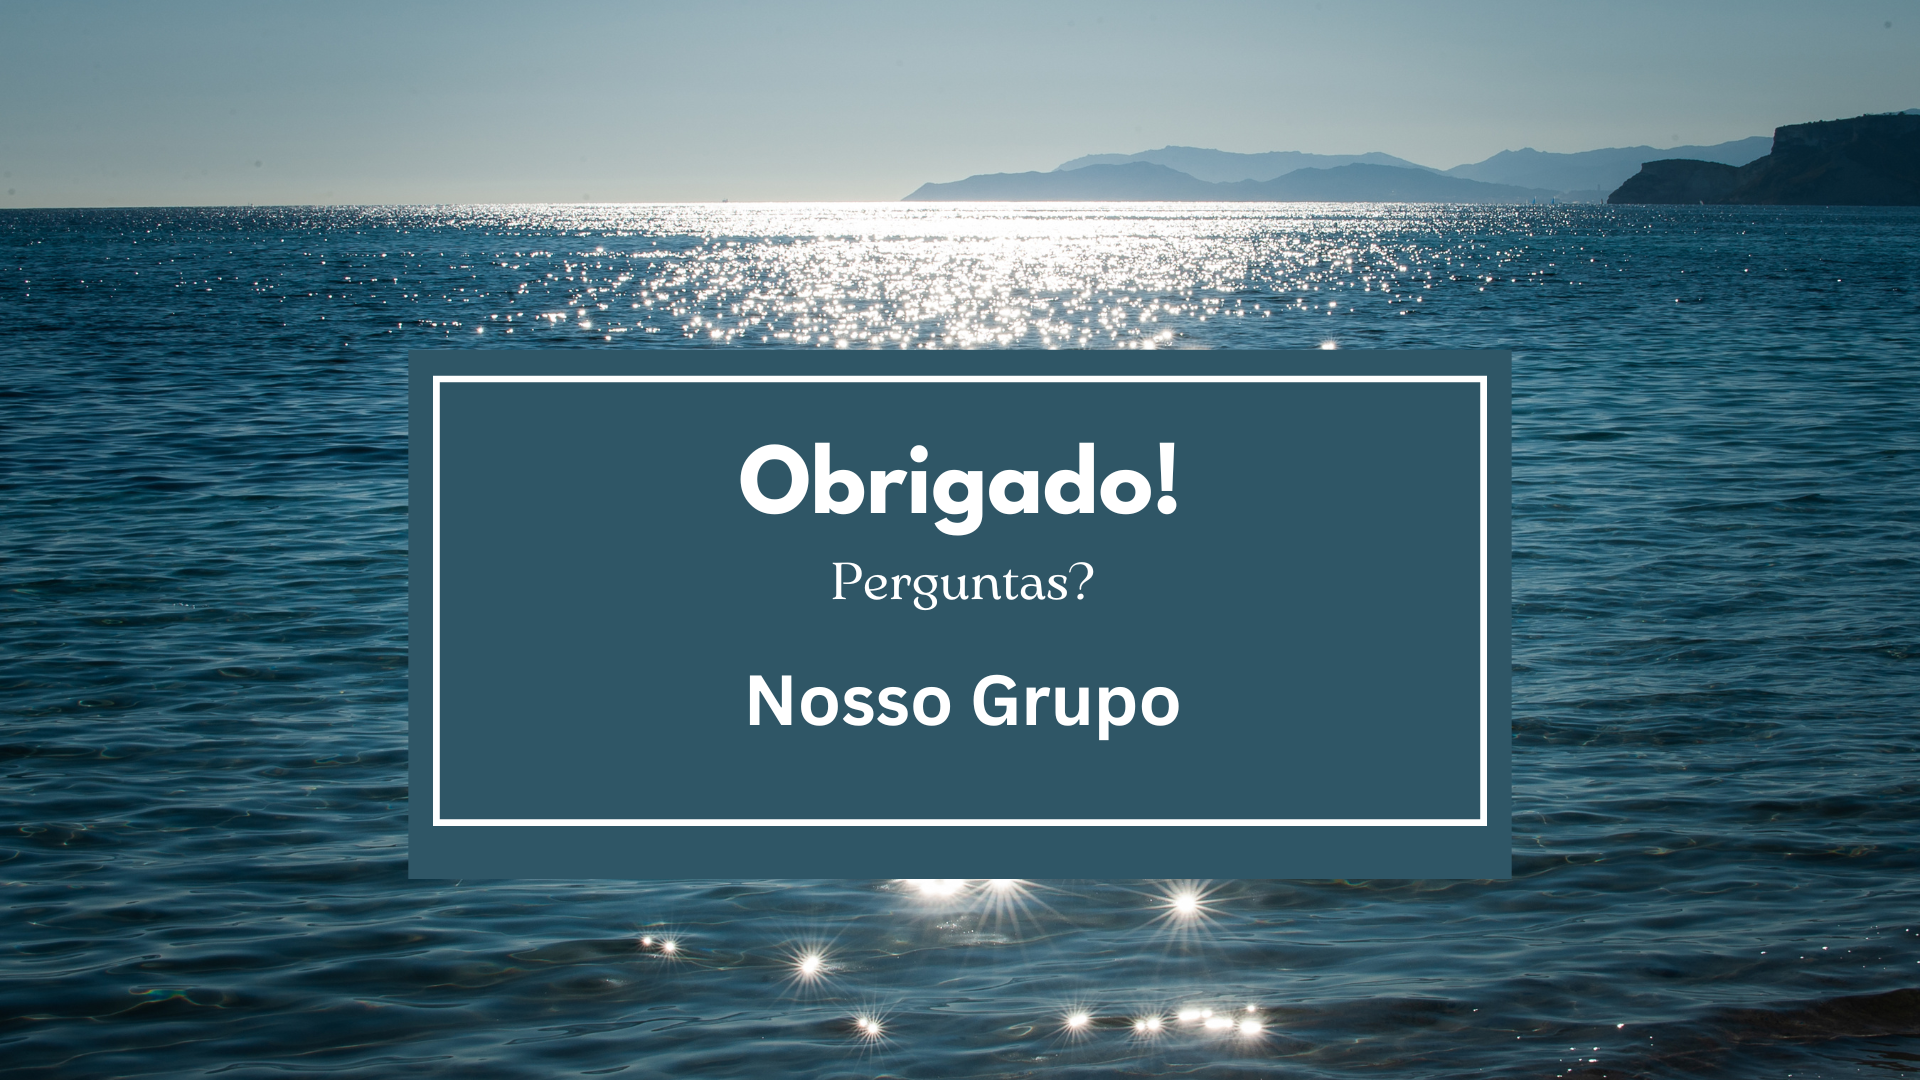
\includegraphics[width=0.87\linewidth,height=0.75\textheight,keepaspectratio]{Obrigado!.png}
\end{frame}

\section{Referências}
\ifcombibliografia
\nocite{briso_atafona_2021}
\nocite{machado2024_dinamica_linha_costa_paraiba_sul}
\nocite{mello2018_erosao_atafona}
\nocite{simcosta_dados_2026}
\nocite{vasconcelos2021_atafona_grussai}
\nocite{asbpa2011_erosion_control_structures}
\nocite{coreloc_imagem}

\begin{frame}[allowframebreaks]{Referências}
  \scriptsize
  \setlength{\bibitemsep}{0pt}
  \setlength{\bibhang}{0pt}
  \renewcommand*{\bibfont}{\scriptsize}
  \printbibliography[heading=none]
\end{frame}
\else
\begin{frame}{Referências principais}
\small
\begin{itemize}
  \item Machado et al. (2024). Dinâmica da linha de costa no flanco meridional do delta do rio Paraíba do Sul.
  \item Vasconcelos et al. (2021). Dinâmica erosiva e progradacional das praias de Atafona e Grussaí.
  \item Mello, Machado e Rocha (2018). Avaliação dos impactos da erosão costeira em Atafona.
  \item SiMCosta (2026). Portal de Dados Meteoceanográficos.
  \item ASBPA (2011). Reintroducing Structures for Erosion Control on the Open Coasts of America.
\end{itemize}
\end{frame}
\fi

\end{document}
